% -----------------
% abnTeX2: Modelo de Trabalho Academico (tese de doutorado, dissertacao de
% mestrado e trabalhos monograficos em geral) em conformidade com 
% ABNT NBR 14724:2011: Informacao e documentacao - Trabalhos academicos -
% Apresentacao
% -----------------

\documentclass[
	% -- opções da classe memoir --
	12pt,                     % tamanho da fonte
	openright,                % capítulos começam em pág ímpar (insere página vazia caso preciso)
	oneside,                  % twoside para impressão em verso e anverso. Oposto a oneside
	a4paper,                  % tamanho do papel. 
  % -- opções da classe abntex2 --
	% chapter=TITLE,          % títulos de capítulos convertidos em letras maiúsculas
	% section=TITLE,          % títulos de seções convertidos em letras maiúsculas
	% subsection=TITLE,       % títulos de subseções convertidos em letras maiúsculas
	% subsubsection=TITLE,    % títulos de subsubseções convertidos em letras maiúsculas
  % -- opções do pacote babel --
	english,                  % idioma adicional para hifenização
	% french,                 % idioma adicional para hifenização
	% spanish,                % idioma adicional para hifenização
	brazil                    % o último idioma é o principal do documento
]{abntex2}

% --- 
% Pacotes básicos 
\usepackage{float}
\usepackage{lmodern}          % Usa a fonte Latin Modern		
\usepackage[T1]{fontenc}      % Selecao de codigos de fonte.
\usepackage[utf8]{inputenc}   % Codificacao do documento (conversão automática dos acentos)
\usepackage{lastpage}         % Usado pela Ficha catalográfica
\usepackage{indentfirst}      % Indenta o primeiro parágrafo de cada seção.
\usepackage{color}            % Controle das cores
\usepackage{graphicx}         % Inclusão de gráficos
\usepackage{microtype}        % para melhorias de justificação
\usepackage[portuges]{datetime2}
\usepackage{makecell}
% \DTMlangsetup[portuges]{showdayofmonth=false}
		
% ---
% Pacotes adicionais, usados apenas no âmbito do Modelo Canônico do abnteX2
\usepackage{lipsum}                           % para geração de dummy text

% ---
% Pacotes de citações
\usepackage[brazilian,hyperpageref]{backref}  % Paginas com as citações na bibl
\usepackage[num]{abntex2cite}                 % Citações padrão ABNT
\citebrackets[]                               % fazer com que as citações dentro do texto virem colchetes
% --- 
% CONFIGURAÇÕES DE PACOTES

% Configurações do pacote backref
% Usado sem a opção hyperpageref de backref
\renewcommand{\backrefpagesname}{Citado na(s) página(s):~}

% Texto padrão antes do número das páginas
\renewcommand{\backref}{}

% Define os textos da citação
\renewcommand*{\backrefalt}[4]{
	\ifcase #1
		Nenhuma citação no texto.
	\or
		Citado na página #2.
	\else
		Citado #1 vezes nas páginas #2.
	\fi}

% ---
% Informações de dados para CAPA e FOLHA DE ROSTO

\titulo{Seleção Dinâmica de Modulação em Redes IEEE 802.15.4/SUN}
\autor{Diego Miranda Medeiros}
\local{Campina Grande}
\data{\the\year{}}
\orientador{Ruan Delgado Gomes}
\newcommand{\instituto}{
  Instituto Federal de Educação, Ciência e Tecnologia\\
  da Paraíba - Campus Campina Grande\\
  Curso Superior de Tecnologia em Telemática
}
\tipotrabalho{Trabalho de conclusão de curso}
% O preambulo deve conter o tipo do trabalho, o objetivo, 
% o nome da instituição e a área de concentração 
\preambulo{Monografia apresentada à Coordenação do Curso de Telemática do IFPB - Campus Campina  Grande,  como  requisito  parcial para conclusão do curso de Tecnologia em Telemática.}

\renewcommand{\imprimircapa}{
  \begin{capa}
    \center

    \begin{figure}
      \begin{center}
        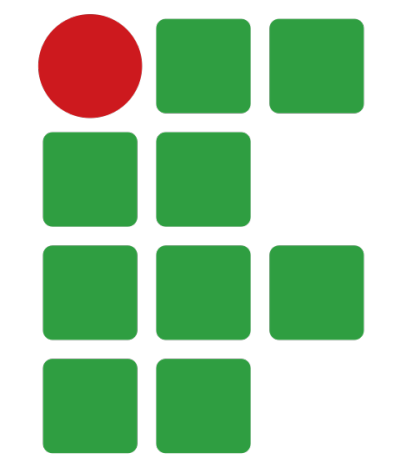
\includegraphics[width=1.8cm]{./assets/logo-ifpb.png}
      \end{center}
    \end{figure}

    \ABNTEXchapterfont \large \MakeUppercase{\instituto}

    \vspace*{2.5cm}

    \ABNTEXchapterfont \large \MakeUppercase{\imprimirautor}

    \vfill
    \begin{center}
      \ABNTEXchapterfont \bfseries \large \MakeUppercase{\imprimirtitulo}
    \end{center}
    \vfill
    % \vspace*{6.25cm}

    \large \imprimirlocal
    \par
    \large \imprimirdata
    \vspace*{1cm}
  \end{capa}
}


% ---
% Configurações de aparência do PDF final

\definecolor{blue}{RGB}{41,5,195}  % alterando o aspecto da cor azul

% informações do PDF
\makeatletter
\hypersetup{
  % pagebackref=true,
  pdftitle={\@title}, 
  pdfauthor={\@author},
  pdfsubject={\imprimirpreambulo},
  pdfcreator={LaTeX with abnTeX2},
  pdfkeywords={abnt}{latex}{abntex}{abntex2}{trabalho acadêmico}, 
  colorlinks=true,          % false: boxed links; true: colored links
  linkcolor=blue,           % color of internal links
  citecolor=blue,           % color of links to bibliography
  filecolor=magenta,        % color of file links
  urlcolor=blue,
  bookmarksdepth=4
}
\makeatother

% --- 
% Espaçamentos entre linhas e parágrafos 

\setlength{\parindent}{1.3cm} % O tamanho do parágrafo

% Controle do espaçamento entre um parágrafo e outro:
\setlength{\parskip}{0.2cm} % Tente também \onelineskip

\makeindex  % Compila o indice

\newcommand{\todo}[1]{{\color{red}[todo] #1}}

% ---
% Início do documento
\begin{document}
\frenchspacing  % Retira espaço extra obsoleto entre as frases.

% ---
% ELEMENTOS PRÉ-TEXTUAIS
% ---
\pretextual
\imprimircapa
\imprimirfolhaderosto*

%% Isto é um exemplo de Ficha Catalográfica, ou ``Dados internacionais de
% catalogação-na-publicação''. Você pode utilizar este modelo como referência. 
% Porém, provavelmente a biblioteca da sua universidade lhe fornecerá um PDF
% com a ficha catalográfica definitiva após a defesa do trabalho. Quando estiver
% com o documento, salve-o como PDF no diretório do seu projeto e substitua todo
% o conteúdo de implementação deste arquivo pelo comando abaixo:
%
% \begin{fichacatalografica}
%     \includepdf{fig_ficha_catalografica.pdf}
% \end{fichacatalografica}

\begin{fichacatalografica}
  \vspace*{\fill}                 % Posição vertical
  \hrule                          % Linha horizontal
  \begin{center}                  % Minipage Centralizado
    \begin{minipage}[c]{12.5cm}   % Largura

      \imprimirautor

      \hspace{0.5cm} \imprimirtitulo  / \imprimirautor. --
      \imprimirlocal, \imprimirdata-

      \hspace{0.5cm} \pageref{LastPage} p. : il. (algumas color.) ; 30 cm.\\

      \hspace{0.5cm} \imprimirorientadorRotulo~\imprimirorientador\\

      \hspace{0.5cm}
      \parbox[t]{\textwidth}{\imprimirtipotrabalho~--~\imprimirinstituicao,
        \imprimirdata.}\\

      \hspace{0.5cm}
      1. Palavra-chave1.
      2. Palavra-chave2.
      I. Orientador.
      II. Universidade xxx.
      III. Faculdade de xxx.
      IV. Título\\

      \hspace{8.75cm} CDU 02:141:005.7\\

    \end{minipage}
  \end{center}
  \hrule
\end{fichacatalografica}
       % Ficha bibliografica
%\begin{errata}
  Elemento opcional da \citeonline[4.2.1.2]{NBR14724:2011}. Exemplo:

  \vspace{\onelineskip}

  FERRIGNO, C. R. A. \textbf{Tratamento de neoplasias ósseas apendiculares com
  reimplantação de enxerto ósseo autólogo autoclavado associado ao plasma
  rico em plaquetas}: estudo crítico na cirurgia de preservação de membro em
  cães. 2011. 128 f. Tese (Livre-Docência) - Faculdade de Medicina Veterinária e
  Zootecnia, Universidade de São Paulo, São Paulo, 2011.

  \begin{table}[htb]
    \center
    \footnotesize
    \begin{tabular}{|p{1.4cm}|p{1cm}|p{3cm}|p{3cm}|}
      \hline
      \textbf{Folha} & \textbf{Linha} & \textbf{Onde se lê} & \textbf{Leia-se} \\
      \hline
      1              & 10             & auto-conclavo       & autoconclavo     \\
      \hline
    \end{tabular}
  \end{table}

\end{errata}
        % Errata
 % Isto é um exemplo de Folha de aprovação, elemento obrigatório da NBR
% 14724/2011 (seção 4.2.1.3). Você pode utilizar este modelo até a aprovação
% do trabalho. Após isso, substitua todo o conteúdo deste arquivo por uma
% imagem da página assinada pela banca com o comando abaixo:
%
% \includepdf{folhadeaprovacao_final.pdf}
%

\begin{folhadeaprovacao}
  \begin{center}
    {\ABNTEXchapterfont\large\imprimirautor}

    \vspace*{\fill}\vspace*{\fill}
    \begin{center}
      \ABNTEXchapterfont \bfseries \Large \imprimirtitulo
    \end{center}
    \vspace*{\fill}

    \hspace{.45\textwidth}
    \begin{minipage}{.5\textwidth}
      \imprimirpreambulo
    \end{minipage}
    \vspace*{\fill}

    % Trabalho aprovado. \imprimirlocal, \today:
  \end{center}

  \assinatura{\textbf{\imprimirorientador} \\ Orientador}
  \assinatura{\textbf{Paulo Ribeiro Lins Junior} \\ Membro da Banca}
  \assinatura{\textbf{Emerson Brasil Gomes } \\ Membro da Banca}
  %\assinatura{\textbf{Professor} \\ Convidado 3}
  %\assinatura{\textbf{Professor} \\ Convidado 4}

  \begin{center}
    \vspace*{0.5cm}
    {\large\imprimirlocal}
    \par
    {\large\imprimirdata}
    \vspace*{1cm}
  \end{center}

\end{folhadeaprovacao}
      % Folha de aprovação
%\begin{dedicatoria}
  \vspace*{\fill}
  \centering
  \noindent
  \textit{ bla bla bla.} \vspace*{\fill}
\end{dedicatoria}
    % Dedicatória
\begin{epigrafe}
  \vspace*{\fill}
  \begin{flushright}
    \textit{'' A fala tem permitido a comunicação de ideias, capacitando os seres humanos a trabalharem juntos para construir o impossível. As maiores conquistas da humanidade surgiram por meio da conversa e seus maiores fracassos por não falar. Não tem que ser assim. Nossas maiores esperanças podem se tornar realidade no futuro. Com a tecnologia à nossa disposição, as possibilidades são ilimitadas. Tudo o que precisamos fazer é garantir que continuamos falando.''\\
      (Pink Floyd - Talkin' Hawkin)}
  \end{flushright}
\end{epigrafe}

      % Epígrafe
\begin{agradecimentos}
\begin{itemize}
    \item Aos meus pais e demais familiares pelo apoio;
    \item Ao meu orientador, Ruan Delgado Gomes, pela oportunidade dada, confiança e dedicação em transmitir seus conhecimentos, além de todo apoio emocional, sou eternamente grato;  
    \item Ao meu co-orientador, Paulo Ribeiro, sempre disponível para ajudar com todo conhecimento possível, além da ajuda dada nesse trabalho, foi de suma importância para o meu crescimento profissional e pessoal;  
    \item A todos que contribuíram com esse trabalho, em especial a Emerson Gomes; 
    \item Ao professor Bruno Jacome, que me deu a primeira oportunidade de participar de um projeto de pesquisa, além de várias contribuições que me ensinaram muito;
    \item Ao GCompi, em especial aos professores Anderson Costa e Jerônimo Rocha;
    \item Ao Assert, em especial ao professor Moacy Pereira, que contribuiu bastante para o meu aprendizado e crescimento profissional;
    \item Aos companheiros de curso, Felipe Ferreira, Marcílio Dantas, Wesley Porto, Daniel Ádonis e Jonathan Barbosa, que me ajudaram bastante durante essa longa caminhada;
    \item À João Manoel, um grande amigo que me ajudou desde o começo do curso, sempre contribuindo para o meu crescimento; 
    \item Aos amigos Arthur Castanha e Natan Dias, que foram de extrema importância para o fechamento deste ciclo;
    \item Aos amigos Romildo Dantas e Luíza Natalle, que me apoiaram bastante durante toda esta caminhada;
    \item A todos os docentes do IFPB-Campus Campina Grande, que contribuíram de forma significativa no meu aprendizado.
     
    
\end{itemize}

\end{agradecimentos}
        % Agradecimentos
% resumo em português
\setlength{\absparsep}{18pt} % ajusta o espaçamento dos parágrafos do resumo
\begin{resumo}
   O uso de redes de sensores na indústria vem crescendo de forma significativa com o passar dos anos, principalmente o uso de redes de sensores sem fio industriais (RSSFIs), devido ás suas vantagens em relação ás redes cabeadas. Entretanto, essas redes carregam um conjunto de desafios, o principal deles é a falta de confiabilidade no canal de comunicação, devido a fontes de interferência e o alto nível de atenuação. Além disso, as RSSFIs apresentam variações nas características do canal ao longo do tempo. Fornecer uma boa qualidade de serviço durante sua operação é de suma importância para implementar uma RSSFI. Este trabalho tem como objetivo dar continuidade a dois trabalhos anteriores que visam melhorar a confiabilidade na comunicação das RSSFIs por meio do uso de diversidade de modulação adaptativa, onde os nós conseguem estimar a qualidade do enlace e decidir a melhor modulação a ser usada no momento. Para isso, foi usado um conjunto de dados obtidos num experimento que utiliza a emenda 'g' do padrão IEEE 802.15.4, padrão esse destinado a redes sem fio pessoais de baixa potência. No experimento chegou-se á conclusão de que nenhuma modulação fornece por si só uma alta taxa de entrega de pacotes na camada de aplicação para todos os nós durante todo o tempo. Esse resultado serviu de base para o desenvolvimento de um mecanismo de modulação adaptativa, que utiliza as três modulações baseadas em uma probabilidade determinada por uma equação e utiliza os pacotes ACK recebidos no transmissor para estimar a qualidade do enlace. Como primeira contribuição, foi proposta uma atualização no mecanismo, que adiciona uma estimação de qualidade de enlace no receptor. A segunda contribuição do trabalho foi juntar os dois estimadores e criar um estimador híbrido, que utiliza das informações obtidas pelos dois estimadores,  criando um mais complexo. Os resultados obtidos por meio de simulações indicam uma melhoria na taxa de entrega de pacotes (PDR) em alguns nós.
   
\vspace{\onelineskip}

  \textbf{Palavras-chaves}: Redes de sensores sem fio industriais, diversidade de modulação, mecanismos de estimação de qualidade de enlace. 
\end{resumo}

% resumo em inglês
\begin{resumo}[Abstract]
  \begin{otherlanguage*}{english}
    The use of sensor networks in the industry has grown significantly over the years, mainly the use of Wireless Sensor Networks (WSNs), due to their advantages over wired networks. However, these networks carry a series of challenges, the main one being the lack of reliability in the communication channel, due to sources of interference and the high level of attenuation. In addition, WSNs are susceptible to variations in channel characteristics over time. Providing a good quality of service during their operation is of paramount importance for implementing WSNs. This work is based on two previous works that aim to improve the reliability of the communication of WSNs through the use of adaptive modulation diversity, where the nodes are able to estimate the quality of the link and decide the best modulation to be used at each moment. For this, we used a dataset obtained in an experiment that uses the 'g' amendment of the IEEE 802.15.4 standard, which is intended for low-power wireless networks. In the experiment it was concluded that no modulation alone provides a high packet delivery ratio at the application layer. This result served as a basis for the development of an adaptive modulation mechanism, which uses the three modulations based on a probability determined by an equation and uses the ACK packets received at the transmitter to estimate the quality of the link. As a first contribution, an update on the mechanism was proposed, in which it adds an estimate of link quality at the receiver. The second and main contribution of the work, was to join the two estimators and create a hybrid estimator, which uses the information obtained by the two estimators and creates a more complex one. The results obtained through simulations indicate an improvement in the packet delivery rate (PDR) in some nodes.

    \vspace{\onelineskip}

    \noindent
    \textbf{Key-words}: Industrial wireless sensor networks, modulation diversity, link quality estimation mechanisms.
  \end{otherlanguage*}
\end{resumo}

% resumo em francês 
% \begin{resumo}[Résumé]
%   \begin{otherlanguage*}{french}
%     Il s'agit d'un résumé en français.

%     \textbf{Mots-clés}: latex. abntex. publication de textes.
%   \end{otherlanguage*}
% \end{resumo}

% % resumo em espanhol
% \begin{resumo}[Resumen]
%   \begin{otherlanguage*}{spanish}
%     Este es el resumen en español.

%     \textbf{Palabras clave}: latex. abntex. publicación de textos.
%   \end{otherlanguage*}
% \end{resumo}
     % Resumos
% ---
% Lista de ilustrações
\pdfbookmark[0]{\listfigurename}{lof}
\listoffigures*
\cleardoublepage

% ---
% Lista de tabelas
\pdfbookmark[0]{\listtablename}{lot}
\listoftables*
\cleardoublepage

% ---
% Lista de abreviaturas e siglas
\begin{siglas}
  \item[RSSF] Redes de Sensores sem Fio
  \item[RSSFI] Redes de Sensores sem Fio Industrial
  \item[ISM] \textit{Industrial, Scientific and Medical}
  \item[MAC] \textit{Media Access Control}
  \item[CSMA/CA] \textit{Carrier Sense Multiple Access with Collision Avoidance}
  \item[TSCH] \textit{Time Slotted Channel Hopping}
  \item[TDMA] \textit{Time Division Multiple Access} 
  \item[FDMA] \textit{Frequency Division Multiple Access}
  \item[SUN] \textit{Smart Utility Network}
  \item[LR-WPAN] \textit{Low Rate Wireless Personal Area Network}
  \item[SUN-FSK] \textit{Frequency-shift keying}
  \item[SUN-OQPSK] \textit{Offset Quadrature Phase-shift keying}
  \item[SUN-OFDM] \textit{Orthogonal Frequency Division Multiplexing}
\end{siglas}

% ---
% Lista de símbolos
%\begin{simbolos}
%  \item[$ \Gamma $] Letra grega Gama
%  \item[$ \Lambda $] Lambda
%  \item[$ \zeta $] Letra grega minúscula zeta
%  \item[$ \in $] Pertence
%\end{simbolos}
         % Listas

% ---
% Sumario
\pdfbookmark[0]{\contentsname}{toc}
\tableofcontents*
\cleardoublepage

% ---
% ELEMENTOS TEXTUAIS
% ---
\textual

% ---
% Introdução (exemplo de capítulo sem numeração, mas presente no Sumário)
\chapter[Introdução]{Introdução}
\label{cap:intro}

Com a chegada da quarta revolução industrial (indústria 4.0), a demanda por monitoramento e controle de processos vem aumentando de forma significativa\cite{klaus}. Esses monitoramentos se dão através de uma rede de sensores, que tradicionalmente, é cabeada. As redes cabeadas apresentam uma maior confiabilidade na conexão, mas apresentam alguns problemas descritos a seguir. O processo de instalação dos cabos possui um custo bastante elevado. Além do custo, redes cabeadas apresentam pouca flexibilidade, o que dificulta a manutenção e futuras expansões da rede\cite{lu2009online}.
 
Uma alternativa que vem ganhando bastante notoriedade são as redes de sensores sem fio (RSSFs). Essas redes carregam várias vantagens em relação a rede cabeada, se destacando o seu baixo custo de instalação, sua flexibilidade e facilidade na implementação e manutenção\cite{gungor2009industrial}. Além dessas vantagens, as RSSFs possuem a capacidade de auto-organização, possibilidade de processamento local e a instalação em locais de difícil acesso ou até mesmo em objetos que se movem constantemente\cite{gomes2017estimaccao}.

Uma RSSF é formada por nós, que podem ser equipados tanto com sensores, quanto com atuadores. Esses nós possuem capacidade de comunicação sem fio (radiofrequência) e em alguns casos, podem ter capacidade de processamento. No caso dos nós com capacidade de processamento, eles conseguem realizar algumas tarefas como o pré-processamento nos dados coletados antes do envio para um nó central(também chamado de nó sorvedouro), dessa forma é possível que o canal de comunicação seja utilizado de forma mais eficiente \cite{sousa2011desafios}. No caso das redes de sensores sem fio industriais(RSSFIs), os sensores são instalados em equipamentos industriais, eles podem realizar tarefas como o monitoramento de temperatura, pressão e vibração\cite{delgado2013impact}. Geralmente, essas informações são encaminhadas através do canal sem fio até uma central, que faz todo esse monitoramento. Com a coleta desses dados, é possível fazer previsões de falhas, observar máquinas que apresentem algum tipo de problema, evitando assim maiores prejuízos\cite{gungor2009industrial}. 

Apesar de todas essas vantagens, as RSSFs carregam uma série de desafios que devem ser levados em conta, o principal deles é a falta de confiabilidade no canal de comunicação. As redes sem fio utilizam um meio de comunicação não confiável, o que pode ser agravado por interferências eletromagnéticas e problemas de atenuação relacionados a sombreamento e multipercurso. Também deve ser levado em conta que esses nós possuem restrições, como baixo poder de processamento e baixa taxa de transmissão\cite{gomes2017estimaccao}. 

No ambiente industrial, esses problemas são agravados. Nesse tipo de ambiente, é possível encontrar várias fontes de interferências, como equipamentos de solda, forno micro-ondas e outros equipamentos que utilizam comunicação sem fio\cite{gomes2014desafios}. Além disso, existem vários objetos metálicos e em grade parte, esses objetos estão se movendo, podendo assim ocasionar uma atenuação do sinal nesse tipo de ambiente\cite{gomes2012correlation}. Esses problemas dificultam a garantia de qualidade de serviço (QoS). Aplicações industriais requerem alta taxa de entrega de pacotes e alta disponibilidade, garantir esse requisitos é de suma importância para implementação de uma RSFFI\cite{gomes2017estimaccao}.

\section{Justificativa e Relevância do Trabalho}
\label{sec:justificativa}

Em \cite{tuset2020evaluating} foi realizado um experimento no período de 99 dias em um ambiente industrial real, em que foi possível avaliar o desempenho de comunicação para 11 nós finais, nas três modulações definidas pelo IEEE 802.15.4g, são elas: SUN-FSK(\textit{Frequency-shift keying}), SUN-OQPSK(\textit{Offset Quadrature Phase-shift keying}) e 
SUN-OFDM(\textit{Orthogonal Frequency Division Multiplexing}). Foi observado que ocorrem variações temporais no desempenho de comunicação de cada modulação e nenhuma modulação consegue individualmente entregar a melhor qualidade de comunicação durante 100 \% do tempo para qualquer um dos nós finais. Foi gerado um conjunto de dados que foi utilizado em \cite{gomes2020improving} para propor mecanismos de diversidade de modulação. Esses mecanismos conseguem identificar a qualidade dos enlaces para cada modulação e escolher a melhor em cada período de tempo, melhorando a taxa da entrega de pacotes e reduzindo o consumo de energia, por meio da redução do número de retransmissões de pacotes. 

Levando em conta os desafios para prover qualidade de serviço em redes sem fio, principalmente em ambientes desafiadores, como a industria, este trabalho tem como objetivo dar continuidade aos dois trabalhos mencionados anteriormente, por meio da proposição de melhorias nos mecanismos de diversidade de modulação para melhorar a qualidade de serviços das redes sem fio que operam em bandas Sub-GHz.   

\section{Objetivos}
\label{sec:objetivo}

\subsection{Objetivo Geral}
\label{subsec:objgeral}

Este trabalho tem como objetivo propor alternativas para melhorar a qualidade de serviços das redes de sensores sem fio por meio de novos mecanismos para escolha dinâmica de modulação, se baseando na emenda IEEE 802.15.4g.

\subsection{Objetivos Específicos}
\label{subsec:objespecificos}

\begin{enumerate}
    \item Estudar as características dos esquemas de modulação do IEEE 802.15.4g e entender suas vantagens e desvantagens e em que situações cada modo de operação pode ser mais adequado;
    \item  Estudar o \textit{dataset} descrito em \cite{tuset2020evaluating} para verificar o desempenho dos três esquemas de modulação avaliados em um ambiente industrial;
    \item Propor algoritmos e mecanismos para estimação de qualidade do enlace, aplicados à identificação das  melhores modulações a serem usadas pelos nós em cada momento;
    \item Avaliar os mecanismos propostos por meio de simulações.
\end{enumerate}

\section{Metodologia}
\label{sec:metodologia}

A metodologia utilizada neste trabalho foi composta pelas seguintes etapas: 

\begin{enumerate}
    \item Levantamento bibliográfico: Nessa etapa foi realizado um estudo de caráter bibliográfico utilizando dois trabalhos que serviram de base\cite{tuset2020evaluating}\cite{gomes2020improving}, com o intuito de compreender aspectos importantes da comunicação sem fio, como o padrão 802.15.4 funciona, padrão esse destinado a redes sem fio pessoais de baixas taxas de transmissão e quais vantagens do uso desse padrão nas redes de sensores. 
    Em seguida, foi realizado um estudo detalhado sobre aspectos importantes para a escolha de modulação a ser usada (ex: presença ou não de fontes de interferência, \textit {link budget} fornecido por cada modulação, etc).
 
    \item  Nessa etapa foi realizada uma análise detalhada do \textit{dataset} descrito em \cite{tuset2020evaluating}. Esse dataset contêm informações referentes a um experimento realizado em um ambiente industrial no período de 99 dias. No experimento, foi implantada uma rede de sensores que utiliza as modulações propostas na emenda 'g' do padrão 802.15.4. Essa análise foi feita com o objetivo de entender os fatores que ocasionaram variações de desempenho para cada modulação no decorrer do tempo. %No experimento foi possível verificar variações temporais no desempenho de comunicação de cada modulação, mostrando que nenhuma modulação agindo individualmente provê a melhor qualidade de comunicação em cem por cento do tempo para qualquer um dos nós finais.
    
    \item Foi feito um estudo no simulador descrito em \cite{gomes2020improving}, que usa as informações do \textit{dataset} para propor estratégias de seleção de modulação adaptativa, com o objetivo de obter a maior taxa de entrega possível. Das estratégias propostas, a estratégia 3M obteve os melhores resultados, a mesma utiliza as três modulações disponíveis no padrão 802.15.g SUN. 
    
    \item Proposta de uma nova estratégia: Nessa etapa foi proposto uma nova estrátegia chamada de 3Mnew, que é uma evolução da 3M\cite{gomes2020improving}. Na estratégia 3M, é utilizado o ARR(\textit{ACK received rate}) para estimar a qualidade do enlace. Observou-se que apesar de ser mais rápida, essa estimação é um pouco falha devido a possibilidade de perca dos pacotes ACK. %A estratégia 3Mnew incrementa uma análise no receptor, que utiliza a taxa de recepção de pacotes(PRR).%
    
    \item Análise detalhada dos estimadores: Nessa etapa foi feita uma análise dos 2 estimadores de qualidade de enlace, com o objetivo de verificar o comportamento dos mesmos e se estão conseguindo estimar com precisão.
    
    \item Nessa etapa foi proposta uma nova abordagem que combina os dois estimadores para formar um estimador mais complexo. 
\end{enumerate}

\section{Organização do Documento}
\label{sec:organizacao}

Os capítulos seguintes estão organizados da seguinte maneira:

O Capítulo 2 apresenta a fundamentação teórica utilizada 
como base para desenvolvimento deste trabalho. São apresentado 
os desafios das RSSFIs, o padrão IEEE 802.15.4g, as três modulações que foram incorporadas ao padrão, o conceito de diversidade de modulação e os trabalhos que serviram de base para essa pesquisa.

O capítulo 3 apresenta os resultados obtidos, onde foi proposto um novo mecanismo de estimação de qualidade do enlace. 

O capítulo 4 apresenta as considerações finais e
 sugestões de trabalhos futuros.




\chapter[Fundamentação Teórica]{Fundamentação Teórica}
\label{cap:Fundamentação Teórica}

\section{Desafios das Redes de Sensores sem Fio Industriais}
\label{sec:desafios}

As RSSFs apresentam uma série de vantagens, destacando o baixo custo e sua flexibilidade. Entretanto, sua implementação carrega uma série de desafios, além de usar um meio de comunicação não confiável, a comunicação sem fio sofre bastante com atenuação e problemas de sombreamento. 
Esses problemas são agravados em ambientes hostis, como é o caso da indústria. Várias fontes de interferência podem ser encontradas em ambientes industriais, geralmente nesses ambientes existem muitos objetos construídos com materias metálicos, robôs, pessoas transitando, entre outros. 
Além disso, as RSSFs utilizam bandas não licenciadas, ocasionando problemas de interferências com outras tecnologias que utilizam a mesma  faixa de frequência\cite{gomes2017estimaccao}.

Dado o constante crescimento no uso de tecnologias que utilizam comunicação sem fio, o espectro disponível acaba ficando mais congestionado e poluído, ocasionando interferências e reduzindo de forma considerável a qualidade de serviço dessas redes que compartilham o mesmo ambiente. A grande maioria desses dispositivos utilizam as faixas de frequência \textit{Industrial, Scientific and Medical}(ISM), que são reservadas internacionalmente para desenvolvimento livre, não possuindo necessidade para licenciamento de utilização de frequência. Alguns dispositivos que não são destinados a comunicação, podem causar interferências nessas faixas, como é o caso do forno micro-ondas\cite{sousa2011desafios}

Em \cite{gomes2012correlation} foi realizado um experimento com o objetivo de avaliar o desempenho do padrão IEEE 802.15.4 em um ambiente industrial. Foi desenvolvida uma investigação da correlação entre a taxa de erro de pacotes e a ocupação espectral, decorrente da interferência de outras fontes que utilizam a mesma faixa dos canais definidos pelo padrão. O resultado mostra como uma nova fonte de interferência pode afetar de forma significativa o desempenho da comunicação. A Figura 1 mostra o impacto de um simples forno micro-ondas ligado perto de um receptor que utiliza o padrão 802.15.4. Em alguns canais, a interferência foi muito alta, resultando em uma taxa de perda de pacote de 50\%, devido ao forno de micro-ondas gerar ruído na mesma faixa de frequência.

\begin{figure}[h]
\label{fig:microondas}
    \caption{\footnotesize Impactado causado por um forno micro-ondas\cite{gomes2012correlation}}
    \centering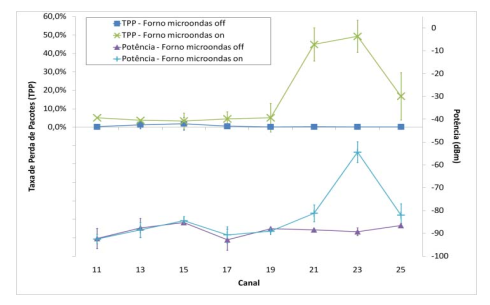
\includegraphics[scale=0.8]{sections/textual/Imagens/experimentoRuan.png}\\
    Fonte \cite{gomes2012correlation}
\end{figure}

\newpage
\section{Padrão IEEE 802.15.4}
\label{sec:padrão}

O padrão 802.15.4 foi lançado inicialmente em 2003 e é destinado para aplicações de redes de sensores sem fio de baixa potência, baixa taxa de transmissão, baixo consumo e baixa complexidade. 

Em 2012, foi lançada a emenda 802.15.4g, que incluiu três novas camadas físicas direcionadas para aplicações SUN \textit{(Smart Utility Network)}, incluindo as modulações: \textit{SUN-FSK}, \textit{SUN-OPQSK} e \textit{SUN-OFDM}~\cite{7460875}. Nesta mesma revisão, foi incluida a menda 802.15.4e que definiu uma camada MAC. O padrão definiu o uso de modos slotted/sincronizado e unslotted/não sincronizado, baseados em CSMA/CA \textit{(Carrier Sense Multiple Access with Collision Avoidance)} para acesso ao meio\cite{gomes2020improving}.

Na revisão IEEE 802.15.4e - 2012 também foi incluído o Salto de canal com intervalo de tempo TSCH(Salto de canal com intervalo de tempo), um mecanisco de acesso ao canal que combina TDMA(Acesso Múltiplo por Divisão de Tempo) e FDMA(Acesso Múltiplo por divisão de Frequência) para suportar requisitos industriais, incluíndo entrega confiável de pacotes. Esse protocolo oferecem maior determinismo em relação ao CSMA/CA, mas sua implementação é mais complexa, pois exige sincronização de tempo entre os nós\cite{gomes2020improving}.


\subsection{SUN-FSK}
\label{subsec:sun-fsk}

A modulação SUN-FSK possuí duas vantagens principais: a primeira é a boa eficiência energética e baixa complexidade de implementação, a segunda é a sua compatibilidade com sistemas legados. A maioria dos sistemas de redes inteligentes implantados 
nos Estados Unidos são baseados nos esquemas de modulação FSK, destacando aqueles que usam a faixa de frequência 902 - 928MHz. 
O SUN-FSK pode ser usado em várias faixas de frequência, o que o torna adequado para diferentes regiões. Três modos de operação diferentes são definidos para cada faixa de frequência, e em cada modo são definidos parâmetros de modulação e canal, 
como o tipo de modulação(2-FSK que fornece uma taxa de transmissão de dados de 50 a 100 kbps e 4-FSK que fornece uma taxa de até 200 kbps), 
o espaçamento do canal e o índice de modulação\cite{tuset2020evaluating}.

Na camada física, o PSDU (\textit{PHY Service Data Unit}) pode ser opcionalmente processado por um codificador Forward Error Correction (FEC).
O FEC pode ser aplicado de duas formas: com código recursivo e sistemático (RSC) ou com código não-recursivo e não sistemático (NRNSC). 
O FEC deve ser empregado no cabeçalho PHY (PHR) e nos bits do PSDU \cite{tuset2020evaluating}.
 
\subsection{SUN-OQPSK}
\label{subsec:sun-oqpsk}

A modulação OQPSK foi incluída no padrão 802.15.4 em 2003, na sua primeira versão. Inicialmente foi definido apenas para a faixa de frequência
de 2.4 Ghz com uma taxa de transmissão de 250 kbps. Posteriormente, outros modos foram definidos, permitindo o uso do OQPSK em outras faixas de
frequência. O SUN-OQPSK emprega o DSSS \textit{(Direct Sequence Spread Spectrum)}, que permite uma melhor resistência a interferências. Essa combinação permite uma taxa de transmissão de até 250 kbps. Existe um modo de espalhamento alternativo, chamado de DSSS multiplexado(MDSSS) e essa combinação permite uma taxa de transmissão que varia de 6,25 kbps até 500 kbps, dependendo do fator de espalhamento\cite{gomes2020improving}.

\subsection{SUN-OFDM}
\label{subsec:sun-ofdm}

O SUN-OFDM foi incluido no padrão 802.15.4g e depois incorporado no 802.15.4 - 2015. Foi incorporado pelo motivo que o OFDM fornece 
altas taxas de dados e longo alcance, ao mesmo tempo que  consegue lidar com problemas de interferência causado por múltiplos caminhos. Apesar dessas 
vantagens, o OFDM carrega algumas dificuldades, pois sua implementação é mais complexa e é necessário um processamento rigoroso, ocasionando um maior
consumo de energia. Vale salientar que o padrão 802.15.4g é voltado para comunicação de baixa potência, consequentemente os equipamentos possuem baixo poder de processamento, e em alguns casos, os mesmos são alimentados por bateria. O SUN-OFDM pode ser usado em diferentes faixas de frequência (sub-GHz e 2,4 GHz) e pode fornecer uma taxa de transmissão de 50 a 800 kbps\cite{tuset2020evaluating}.

\section{Diversidade}
\label{sec:diversidade}

Tanto o \textit{fading} quanto o sombreamento induzem uma penalidade bem significativa no desempenho da modulação em canais sem fio. Um técnica bem eficiente que pode mitigar esses efeitos de forma significativa, é o uso de diversidade \cite{goldsmith2005wireless}. A diversidade é uma técnica usada para compensar os danos causados pela atenuação no canal, sem a necessidade de aumentar a potência ou a largura de banda transmitida e permitindo a configuração do canal, modulação, rotas diferentes, etc. A técnica de diversidade mais conhecida é a diversidade espacial\cite{rappaport2009}, nela é necessário o uso de múltiplas antenas, que são espaçadas estrategicamente e conectadas a um sistema. Se por um acaso uma das antenas captar um sinal nulo, as outras antenas podem captar um pico do sinal e o receptor ser capaz de selecionar a antena com a melhor recepção naquele determinado momento. 

\subsection{Diversidade de Modulação} A diversidade de modulação tem como objetivo melhorar a confiabilidade das comunicações usando diferentes modulações. A ideia é que pacotes consecutivos possam ser transmitidos usando duas ou mais modulações, buscando vantagens em relação a propagação e interferências. Esse conceito não é algo novo, mas o uso de diversidade de modulação foi limitado devido a indisponibilidade de transceptores comerciais que suportassem múltiplas modulações. Com o surgimento do padrão IEEE 802.15.4g e a disponibilidade de transceptores, o uso da diversidade de modulação em redes sem fio de baixa potência pode ser explorado. 

Várias estratégias podem ser usadas para implementar esse conceito, dependendo de qual lado vai tomar a decisão de que modulações devem ser usadas por cada nó. Os mecanismos de estimação podem fazer uso dos estimadores de qualidade de enlace. No nó transmissor, pode ser usado como métrica o \textit{ACK Reception Ratio}(ARR). O ARR é o resultado da razão entre o número de ACKs recebidos com sucesso e o número de pacotes transmitidos em um determinado intervalo de tempo. Já no lado do receptor, pode ser usado o \textit{packet receiving rate}(PRR). O PRR é a razão entre pacotes recebidos com sucesso pelo receptor e os pacotes transmitidos pelo transmissor de acordo com uma janela especificada. O uso de diversidade de modulação pode ser de forma fixa, onde é definida que modulação usar no momento, a partir de um conjunto fixo ou de forma adaptativa. No caso da modulação adaptativa, é necessário que o canal de comunicação possa ser estimado, a partir disso, os nós conseguem visualizar a qualidade do enlace e decidir que modulação é melhor em determinado momento\cite{gomes2020improving}. A modulação adaptativa também não é um conceito novo, essa estratégia foi sugerida pela primeira vez no final dos anos sessenta. Infelizmente tiveram vida curta, devido a restrições de \textit{hardware} e pela falta de uma técnica que conseguisse fornecer uma estimativa do canal eficiente e precisa\cite{goldsmith2005wireless}.

\section{Trabalhos Relacionados}
\label{sec:trabrelacionados}

Em \cite{tuset2020evaluating} foi realizado um experimento no período de 99 dias onde 11 nós \textit{OpenMote-B} foram distribuídos em um ambiente industrial real. Foi implementada uma rede de sensores que utiliza uma topologia estrela e os nós foram distribuídos em distâncias que variam de 34~m a 274~m em relação ao \textit{gateway}.
Cada nó em um intervalo de 1 minuto gera um pacote e envia usando cada modulação SUN. Esses pacotes foram enviados três vezes usando cada modulação (9 transmissões no total). O \textit{gateway} foi equipado com três transceptores de rádio IEEE 802.15.4g  independentes para poder receber pacotes de forma simultânea. Como parâmetro de avaliação, foi utilizado o PDR(taxa de entrega de pacotes). 

No experimento, foi observado que nenhuma modulação consegue por si só fornecer uma alta taxa de entrega de pacotes na camada de aplicação. Aplicações industriais necessitam de uma alta taxa de entrega (PDR > 99.9\%). No experimento, essa taxa foi obtida devido a replicação de pacotes(3 transmissões usando cada modulação, 9 no total). Vale salientar que essa técnica pode sobrecarregar a rede, pois o alto número de transmissões aumenta de forma significativa o consumo de energia no nó, limitando sua durabilidade, caso o mesmo seja alimentado por bateria e podendo limitar a escalabilidade da rede.

Dando continuidade ao trabalho anterior, em \cite{gomes2020improving}, foi proposta a utilização de três estratégias de seleção de modulação adaptativa(denominadas 1M, 2M e 3M) com o objetivo de melhorar a confiabilidade do enlace nas redes IEEE 802.15.4g. 
A métrica usada para estimar a qualidade do enlace foi o ARR. O ARR é calculado a partir da razão entre o número de pacotes ACKs recebidos com sucesso e o número de pacotes transmitidos em um determinado intervalo de tempo.    

A estratégia 1M usa apenas uma modulação do IEEE 802.15.4g para permitir que os nós transmitam pacotes. Quando a qualidade do enlace cai abaixo de um limiar determinado, a modulação é trocada seguindo uma ordem. A 2M usa duas das três modulações, são nomeadas como m1 e m2, respectivamente. Por exemplo, m1 está usando SUN-FSK nas tentativas impares e m2 usando SUN-OQPSK nas tentativas pares, se a qualidade do SUN-FSK cai abaixo de um limiar, SUN-OPQSK vira m1 e SUN-OFDM que estava aguardando, vira m2. Tanto no 1M quanto no 2M, foi considerado um limiar de 0.9 no valor do ARR para acontecer a troca das modulações. E por último, a estratégia 3M, na qual se obteve os melhores resultados, mostrando a importância do uso de diversividade de modulação. A estratégia 3M usa as três modulações para permitir que os nós possam transmitir pacotes, cada nó seleciona uma modulação com base em uma probabilidade, determinada por uma equação. Essas probabilidades são calculadas periodicamente com base na qualidade dos enlaces e sempre que uma nova estimativa da qualidade do enlace calculada para uma das modulações, a probabilidade de uso das outras modulações também são atualizadas.

Para avaliar as estratégias mencionadas, foi desenvolvido um simulador em Python, que usa os valores de PDR do \textit{dataset} descrito em \cite{tuset2020evaluating}. O simulador usa o conjunto de dados para calcular o PDR na camada física de todas as modulações e nós a cada 5 minutos. Com base nos valores de PDR calculados, o simulador determina se cada pacote transmitido e seu reconhecimento(ACK) é entregue ou não. Quando um ACK não for recebido, devido a uma falha em uma das duas transmissões(pacotes ou ACKs), o nó pode retransmitir o mesmo pacote, de acordo com um número de tentativas permitidas.

Além das estratégias de seleção de modulação mencionadas, foram implementadas três estratégias para servir de comparação: \textit{Round-Robin}, onde os nós usam as modulações de maneira alternada, \textit{Random}, onde os nós usam as três modulações de forma aleatória com probabilidades iguais e a \textit{Best}, onde é simulado o maior PDR alcançado caso os nós sempre consigam usar a melhor modulação
o tempo todo, essa estratégia representa um limite superior, dada as condições do canal.

As métricas usadas para avaliar o desempenho das estratégias de modulação propostas são o PDR e o RNP (número necessário de transmissões de pacotes). O PDR é calculado pela razão entre pacotes recebidos e transmitidos, a RNP representa o número médio de repetições de pacotes antes de uma recepção bem sucedida. A RNP e o PDR são complementares para avaliar a qualidade do enlace. Menores valores de RNP indicam que a maioria dos pacotes foi entregue na primeira tentativa de transmissão. Os códigos fonte referentes ás estratégias estão disponíveis em \cite{gitGcompi}.

\chapter{Mecanismos de Diversidade de Modulação Propostos}
\label{sec:mecanismos}

Como mencionado anteriormente, este trabalho tem como objetivo dar continuidade a dois trabalhos. Em \cite{tuset2020evaluating} Onde foi obtido um conjunto de dados com informações da taxa de entrega de pacotes proveniente de 11 nós e em \cite{gomes2020improving} onde foram propostos mecanismos de diversidade de modulação para obter uma melhor taxa de entrega de pacotes. A melhor estratégia proposta foi a 3M, onde se usa as três modulações baseadas em uma equação de probabilidade para determinar a melhor modulação a ser usada em determinado momento. Antes de transmitir um pacote, cada nó seleciona uma modulação com base na probabilidade de uso, segue a equação: \ref{eq:3M}

\begin{equation}
\label{eq:3M}
p_i = \frac{{(1+a_i)}^w}{\sum_{k=0}^{k<3}{(1+a_k)}^w},
\end{equation}

em que $p_i$ é a probabilidade de usar a modulação \textit{i} (onde 0 é SUN-FSK, 1 é SUN-OQPSK e 2 é SUN-OFDM), $a_i$ é o valor do ARR para a modulação \textit{i} e \textit{w} é um fator de peso usado para controlar as diferenças entre os valores de probabilidades calculados. Se uma tentativa de transmissão a falhar, a retransmissão de pacotes não pode usar a mesma modulação. Em vez disso, a modulação a ser usada é selecionada entre as demais de acordo com suas probabilidades. Dessa forma é permitido aumentar a diversidade. É possível observar que essas probabilidades são calculadas periodicamente com base na qualidade dos enlaces e sempre que um novo valor é calculado para uma das modulações, as probabilidades das outras também são atualizadas. O ARR para uma determinada modulação é calculado com base apenas nos pacotes transmitidos usando esta modulação, então quando uma probabilidade tem um \textit{p} alto, seu ARR é atualizado com mais frequência. Se a qualidade de um link para uma determinada modulação que tem um valor de \textit{p} alto  cai, as probabilidade serão ajustadas rapidamente. Se a modulação com \textit{p} baixo começar a apresentar boa qualidade, levará mais tempo até que as probabilidades sejam ajustadas. 

A partir disso, foram realizadas análises sobre a possibilidade de melhorar esse mecanismo. Foi possível observar que o método de estimação de qualidade do enlace do 3M \cite{gomes2020improving} possui uma limitação. Apesar do ARR conseguir fornecer estimativas de forma rápida e não utilizar o canal de comunicação para fazer essa estimativa, o canal sem fio pode apresentar assimetria, de modo que um determinado pacote pode ter chegado no receptor, mas a entrega do pacote ACK pode vir a falhar, em termos gerais, esse pacote foi entregue, mas como a análise é feita no transmissor, esse pacote é considerado como perdido, mas na prática, o mesmo foi entregue. A Figura \ref{fig:transm} mostra uma transmissão entre um transmissor e um receptor. 

\begin{figure}[H]
    \caption{\footnotesize Representação de uma transmissão entre um transmissor e um receptor}
    \centering
    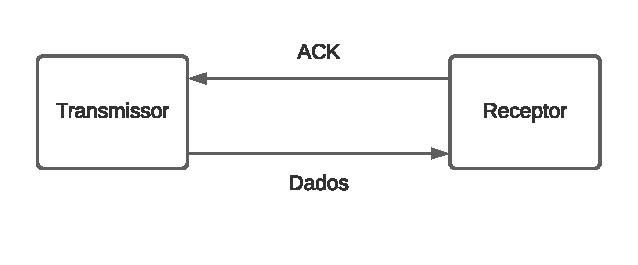
\includegraphics[scale = 0.9]{sections/textual/Imagens/diagrama.pdf}\\
    Fonte autoral
    \label{fig:transm}
\end{figure}

\section{3Mnew}

Como primeira contribuição, foi proposta uma atualização no mecanismo 3M, chamada de 3M\textit{new}, onde é adicionado no receptor, uma análise para calcular a qualidade do enlace. O receptor realiza esta análise usando o PRR, que faz o cálculo da seguinte forma: quantidade de pacotes recebidos dividido pela quantidade de pacotes enviados em uma determinada janela para cada modulação. Foram avaliadas janelas contendo entre 6 e 11 pacotes. Após as simulações, observou-se que com uma janela de 9 pacotes, é possível obter um resultado ligeiramente melhor. 
Na Tabela~\ref{tabela:janela} são mostrados os valores de PDR médio global utilizando cada tamanho de janela.


\begin{table}[H]
\centering
\begin{tabular}{|l|l|l|l|l|l|l|}
\hline
Tamanho da janela   & 6  & 7  & 8  & 9  & 10  & 11  \\ \hline
PDR(\%) & 97.88  & 97.88  & 97.88  & 97.89  & 97.87   & 97.87   \\ \hline
MAX(\%) & 99.74  & 99.74  & 99.74  & 99.76  & 99.74   & 99.74   \\ \hline
MIN(\%) & 93.05  & 93.04  & 93.02  & 93.06  & 93.01   & 93.03   \\ \hline
\end{tabular}
\caption{Resultado da variação da janela de pacotes para o cálculo do PRR}
\label{tabela:janela}
\end{table}

Após realizar o cálculo do PRR, é feita uma análise se o valor encontrado é diferente do PRR encontrado na janela anterior, se sim, é enviado um sinal(por meio de um bit no pacote ACK
) para o transmissor, que realiza a atualização das probabilidades de uso de cada modulação, de acordo com a equação 3M(Equação\ref{eq:3M}), considerando o valor do PRR no lugar do valor do ARR para determinar as probabilidades das modulações a serem escolhidas. A equação \ref{eq:3Mnew} mostra a mudança em relação ao 3M(Equação\ref{eq:3M}), onde o $prr_i$ é valor do PRR para a modulação \textit{i}. O código fonte do 3M\textit{new} está disponível em \cite{GitDiego}.
\begin{equation}
\label{eq:3Mnew}
p_i = \frac{{(1+prr_i)}^w}{\sum_{k=0}^{k<3}{(1+prr_k)}^w}
\end{equation}

\begin{figure}
    \centering
    \caption{Funcionamento do 3M\textit{new}}
    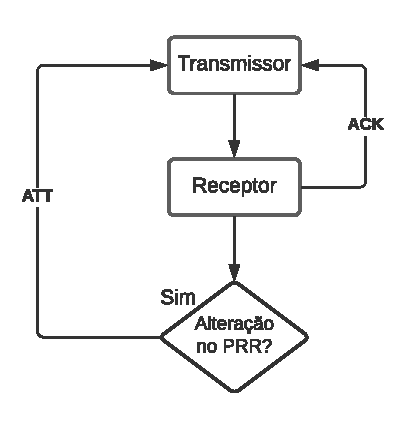
\includegraphics{sections/textual/Imagens/3Mnew.pdf} \\ Fonte autoral
    \label{fig:3Mnew}
\end{figure}

\newpage
\section{3Mh}

Após a análise feita nos estimadores, descrito na seção \ref{res:estimadores}, foi possível observar que apesar dos estimadores conseguirem se aproximar dos valores reais, ambos não conseguem realizar a estimação de forma precisa em 100\% do tempo. Foi chegada à conclusão que um estimador mais complexo que conseguisse usar os dois valores para obter a estimação do enlace poderia ser sair melhor, se aproveitando das vantagens que ambos podem oferecer. 

Essa nova abordagem é realizada no transmissor, utilizando os valores combinados do ARR e PRR com pesos iguais. Nessa estratégia, é mantida a ideia do 3M\textit{new}, onde o receptor também faz a análise da qualidade do enlace de forma independente, e caso tenha alteração no PRR em relação á janela anterior, o mesmo recalcula as probabilidades. Segue Equação: \ref{eq:3Mh}. O código fonte do 3Mh está disponível em \cite{GitDiego}. 

\begin{equation}
\label{eq:3Mh}
	p_i = \frac{{(1+((arr_i\times0.5) + (prr_i\times0.5)))}^w}{\sum_{k=0}^{k<3}{(1+((arr_k\times0.5) + (prr_k\times0.5))}^w}
\end{equation}

\chapter{Resultados}

\section{Metodologias de Avaliação}
\label{res:parâmestros}

\subsection{Métricas}

As métricas usadas para avaliar o desempenho das estratégias de modulação propostas são o PDR na camada de aplicação e o RNP (\textit{Required Number of Packet transmissions}). O PDR é calculado pela razão entre pacotes recebidos e transmitidos na camada de aplicação (ou seja, independente se houve retransmissão ou não), enquanto que a RNP representa o número médio de repetições de pacotes antes de uma recepção bem sucedida. A RNP e o PDR são complementares para avaliar a qualidade dos enlaces. Menores valores de RNP indicam que a maioria dos pacotes foi entregue na primeira tentativa de transmissão.

\subsection{Configurações de simulação}

Para avaliar as estratégias mencionadas, foi usado um simulador escrito em Python, descrito em~\cite{gomes2020improving}, que utiliza o conjunto de dados descritos em~\cite{tuset2020evaluating} para calcular o PDR na camada física de todas as modulações e nós a cada 5 minutos. Com base nos valores de PDR calculados, o simulador determina se cada pacote transmitido e seu reconhecimento (ACK) é entregue ou não. Quando um ACK não for recebido, devido a uma falha em uma das duas transmissões (pacotes ou ACKs), o nó pode retransmitir o mesmo pacote, de acordo com um número máximo de tentativas permitidas. O simulador foi estendido para dar suporte também às duas novas estratégias de estimação de qualidade de enlace propostas neste trabalho (3M\textit{new} e 3Mh). Para obter os resultados descritos neste trabalho, foram feitas 10 simulações para cada nó e obtido o valor médio do PDR e da RNP. Foi permitido o uso de até 6 retransmissões de pacotes.  

\section{Análise dos estimadores}
\label{res:estimadores}

Após a avaliação da estratégia proposta (3M\textit{new}), o próximo passo foi avaliar a precisão dos estimadores, fazendo um comparativo com o PDR do \textit{dataset} \cite{tuset2020evaluating}. Tanto da estratégia 3M, que utiliza o ARR como métrica, quanto da 3M\textit{new}, que utiliza o ARR e o PRR. 

Essa avaliação foi feita em duas etapas. Primeiro foi feita a análise entre o ARR e o PDR encontrado no dataset \cite{tuset2020evaluating} para cada modulação. Vale salientar que o valor do PDR é o valor real encontrado no experimento, então ele serve como base para analisar a precisão dos estimadores. Na segunda etapa foi feita a análise do PRR com o PDR. 

Para chegar nesses resultados, foi desenvolvido um simulador em 
Python, que após 10 simulações, organiza em um mesmo vetor os valores médios obtidos de cada estimador(ARR, PRR e o híbrido) para cada um dos 11 nós e também para cada modulação(SUN-FSK, SUN-OQPSK e SUN-OFDM). A partir disso, é calculado o erro quadrático médio em relação ao PDR, onde o valor mais próximo do zero, indica uma melhor precisão do estimador. O código fonte do simulador esta disponível em \cite{GitDiego}.

Como pode-se observar, os estimadores conseguem se aproximar dos valores reais obtidos. O PRR se sai melhor que o ARR, devido o fato que o PRR não leva em consideração os pacotes ACKs que podem ser perdidos antes de chegar no transmissor. Por outro lado, o ARR consegue os valores de estimação de forma mais rápida, tendo em vista que todos esses cálculos de probabilidade dos mecanismos, são realizados no transmissor e o mesmo não utiliza o canal de comunicação para realizar essa estimação. 

As tabelas ~\ref{tab:est1}, ~\ref{tab:est2} e ~\ref{tab:est3} mostram os valores do erro quadrático médio para os 11 nós e para cada modulação. A tabela \ref{tab:est3} mostra os valores do mecanismo de estimação usado na estratégia 3Mh, que utiliza os valores combinados do ARR e PRR com pesos iguais. Como pode-se observar, o PRR se sai melhor em todos os nós e em todas as modulações. A estimação híbrida proposta, não consegue superar a precisão do PRR, no entanto, consegue se aproximar. Apesar do PRR fornecer uma estimação mais precisa, não foi possível obter um melhor PDR utilizando esse método de estimação de forma isolada. A vantagem que o ARR fornece em não utilizar o canal de comunicação para a troca de dados é bastante relevante, tendo em vista que a decisão de usar determinada modulação é realizada no transmissor. 

\begin{table}[H]
\centering
\begin{tabular}{|c|ccc|}
\hline
\multicolumn{1}{|c|}{}     & \multicolumn{1}{c|}{arr-fsk} & \multicolumn{1}{c|}{prr-fsk} & \multicolumn{1}{c|}{h-fsk}  \\ \hline
\multicolumn{1}{|c|}{5653} & \multicolumn{1}{c}{0.3785}   & \multicolumn{1}{c}{0.2816}   & \multicolumn{1}{c|}{0.3146} \\ \cline{1-1}
55ad & 0.2939 & 0.2109 & 0.2333 \\ \cline{1-1}
55e4 & 0.3299 & 0.2275 & 0.2536 \\ \hline
5599 & 0.3083 & 0.2522 & 0.2644 \\ \cline{1-1}
55dd & 0.5329 & 0.4406 & 0.4829 \\ \cline{1-1}
5565 & 0.4374 & 0.3055 & 0.3538 \\ \cline{1-1}
560b & 0.4841 & 0.4228 & 0.4539 \\ \hline
5632 & 0.3198 & 0.2496 & 0.2826 \\ \cline{1-1}
55b3 & 0.3834 & 0.2775 & 0.3065 \\ \cline{1-1}
5563 & 0.2135 & 0.1687 & 0.1654 \\ \cline{1-1}
630a & 0.3394 & 0.2769 & 0.3005 \\ \hline
\end{tabular}
\caption{Análise dos estimadores da modulação FSK}
\label{tab:est1}
\end{table}

\begin{table}[H]
\centering
\begin{tabular}{|c|ccc|}
\hline
\multicolumn{1}{|c|}{}     & \multicolumn{1}{c|}{arr-oqpsk} & \multicolumn{1}{c|}{prr-oqpsk} & \multicolumn{1}{c|}{h-oqpsk} \\ \hline
\multicolumn{1}{|c|}{5653} & \multicolumn{1}{c}{0.4556}     & \multicolumn{1}{c}{0.3776}     & \multicolumn{1}{c|}{0.4012}  \\ \cline{1-1}
55ad & 0.5863 & 0.5109 & 0.5445 \\ \cline{1-1}
55e4 & 0.4348 & 0.3682 & 0.3847 \\ \hline
5599 & 0.2930 & 0.2184 & 0.2306 \\ \cline{1-1}
55dd & 0.5119 & 0.4896 & 0.4968 \\ \cline{1-1}
5565 & 0.3338 & 0.2335 & 0.2695 \\ \cline{1-1}
560b & 0.4977 & 0.4698 & 0.4797 \\ \hline
5632 & 0.5547 & 0.3965 & 0.4815 \\ \cline{1-1}
55b3 & 0.3698 & 0.3108 & 0.3288 \\ \cline{1-1}
5563 & 0.6420 & 0.6049 & 0.6092 \\ \cline{1-1}
630a & 0.3559 & 0.2605 & 0.2914 \\ \hline
\end{tabular}
\caption{Análise dos estimadores da modulação OQPSK}
\label{tab:est2}
\end{table}

\begin{table}[H]
\centering
\begin{tabular}{|c|ccc|}
\hline
\multicolumn{1}{|c|}{}     & \multicolumn{1}{c|}{arr-ofdm} & \multicolumn{1}{c|}{prr-ofdm} & \multicolumn{1}{c|}{h-ofdm} \\ \hline
\multicolumn{1}{|c|}{5653} & \multicolumn{1}{c}{0.5234}    & \multicolumn{1}{c}{0.4315}    & \multicolumn{1}{c|}{0.4618} \\ \cline{1-1}
55ad & 0.3804 & 0.2983 & 0.3234 \\ \cline{1-1}
55e4 & 0.4463 & 0.3194 & 0.3699 \\ \hline
5599 & 0.5189 & 0.4026 & 0.4427 \\ \cline{1-1}
55dd & 0.4489 & 0.3199 & 0.3696 \\ \cline{1-1}
5565 & 0.6799 & 0.6235 & 0.6405 \\ \cline{1-1}
560b & 0.4583 & 0.3656 & 0.3921 \\ \hline
5632 & 0.6370 & 0.6016 & 0.6029 \\ \cline{1-1}
55b3 & 0.6600 & 0.5509 & 0.5960 \\ \cline{1-1}
5563 & 0.4230 & 0.3671 & 0.3848 \\ \cline{1-1}
630a & 0.4153 & 0.3625 & 0.3823 \\ \hline
\end{tabular}
\caption{Análise dos estimadores da modulação OFDM}
\label{tab:est3}
\end{table}

As figuras \ref{fig:graf1}, \ref{fig:graf2} e \ref{fig:graf3} mostram o comparativo dos três estimadores usados nesse trabalho, ARR, PRR e o estimador híbrido proposto, com o PDR encontrado no dataset  \cite{tuset2020evaluating} para a modulação SUN-FSK no primeiro nó, o 5653. Como pode-se observar, o PRR consegue estimar melhor, a estimação híbrida consegue se aproximar do PRR. Apesar do PRR fornecer uma estimação mais precisa, o híbrido consegue fornecer um PDR superior, como mostrado na seção \ref{resultados}. A vantagem do ARR em não usar o canal de comunicação se mostrou bastante relevante. 

\begin{figure}[H]
    \centering
    \caption{\footnotesize Análise de estimação, ARR e PDR, da modulação SUN-FSK}
    
\includegraphics[scale = 0.08]{sections/textual/Imagens/5653_arr_fsk.pdf}\\
    Fonte: Autoria própia
    \label{fig:graf1}
\end{figure}

\begin{figure}[H]
    \centering
    \caption{\footnotesize Análise de estimação, PRR e PDR, modulação SUN-FSK}
    
\includegraphics[scale = 0.08]{sections/textual/Imagens/5653_prr_fsk.pdf}\\
    Fonte: Autoria própia
    \label{fig:graf2}
\end{figure}

\begin{figure}[H]
    \centering
    \caption{\footnotesize Análise de estimação, híbrido e PDR, modulação SUN-FSK}
    
\includegraphics[scale = 0.08]{sections/textual/Imagens/5653_h_fsk.pdf}\\
    Fonte: Autoria própia
    \label{fig:graf3}
\end{figure}

\newpage
As figuras \ref{fig:graf4}, \ref{fig:graf5} e \ref{fig:graf6} mostram os comparativos dos três estimadores para a modulação SUN-OQPSK no primeiro nó, o 5653. O comportamento se repete em relação ao SUN-FSK, onde o PRR consegue estimar melhor, o híbrido consegue de certa forma se aproxima. Algumas quedas bruscas podem ser observadas no mesmo período de tempo nos três estimadores, o motivo dessas quedas serão avaliadas em trabalhos futuros. 

\begin{figure}[H]
    \centering
    \caption{\footnotesize Análise de estimação, ARR e PDR, modulação SUN-OQPSK}
    
\includegraphics[scale = 0.08]{sections/textual/Imagens/5653_arr_oqpsk.pdf}\\
    Fonte: Autoria própia
    \label{fig:graf4}
\end{figure}

\begin{figure}[H]
    \centering
    \caption{\footnotesize Análise de estimação, PRR e PDR, modulação SUN-OQPSK}
    
\includegraphics[scale = 0.08]{sections/textual/Imagens/5653_prr_oqpsk.pdf}\\
    Fonte: Autoria própia
    \label{fig:graf5}
\end{figure}

\begin{figure}[H]
    \centering
    \caption{\footnotesize Análise de estimação, híbrido e PDR, modulação SUN-OQPSK}
    
\includegraphics[scale = 0.08]{sections/textual/Imagens/5653_h_oqpsk.pdf}\\
    Fonte: Autoria própia
    \label{fig:graf6}
\end{figure}

As figuras \ref{fig:graf7}, \ref{fig:graf8} e \ref{fig:graf9} mostram os comparativos dos três estimadores para a modulação SUN-OFDM no primeiro nó, o 5653. É possível observar que nenhum estimador consegue fornecer estimativas no início, isso se da ao fato de que as modulações são escolhidas baseadas numa probabilidade, para o estimador conseguir calcular, essa modulação deve ser escolhida. Nesse caso, ou o OFDM não foi escolhida devido ao fato que a mesma não estava fornecendo uma boa confiabilidade neste momento, ou as outras duas modulações disponíveis (SUN-FSK e SUN-OQPSK) estavam se saindo melhor que a OFDM. 


\begin{figure}[H]
    \centering
    \caption{\footnotesize Análise de estimação, ARR e PDR, modulação SUN-OFDM}
    
\includegraphics[scale = 0.08]{sections/textual/Imagens/5653_arr_ofdm.pdf}\\
    Fonte: Autoria própia
    \label{fig:graf7}
\end{figure}

\begin{figure}[H]
    \centering
    \caption{\footnotesize Análise de estimação, PRR e PDR, modulação SUN-OFDM}
    
\includegraphics[scale = 0.08]{sections/textual/Imagens/5653_prr_ofdm.pdf}\\
    Fonte: Autoria própia
    \label{fig:graf8}
\end{figure}

\begin{figure}[H]
    \centering
    \caption{\footnotesize Análise de estimação, híbrido e PDR, modulação SUN-OFDM}
    
\includegraphics[scale = 0.08]{sections/textual/Imagens/5653_h_ofdm.pdf}\\
    Fonte: Autoria própia
    \label{fig:graf9}
\end{figure}

 Os valores das estimações e as análises gráficas dos outros 10 nós, estão disponíveis em \cite{GitDiego}. 


\section{Resultados das propostas}
\label{resultados}

Além das duas estratégias propostas neste trabalho, foram usadas as estratégias propostas em \cite{gomes2020improving} como comparativo (1M, 2M, 3M, \textit{Random}, \textit{round-robin}, \textit{best}). Para uma melhor análise dos resultados, os nós foram divididos em três grupos, de acordo com a distância entre os nós e o \textit{gateway}. 

\begin{itemize}
\item Grupo 1 ($d < 80$~m - Nós: 5653, 55ad, 55E4); 
\item Grupo 2 (80~m $\le$ $d < 150$~m - Nós: 5599, 55dd, 5565, 560b);
\item Grupo 3 ($d \ge 150$~m - Nós: 5632, 55b3, 5563, 630a).
\end{itemize}

As figuras \ref{fig:g1}, \ref{fig:g2} e \ref{fig:g3} mostra o PDR para os grupos 1, 2 e 3, respetivamente. Através dos gráficos, é possível observar que a segunda estratégia proposta, 3Mh, consegue um PDR superior em 9 dos 11 nós, indicando que o uso de diversidade de modulação melhora a confiabilidade do canal, ou seja, o PDR. Em alguns nós, o uso de apenas uma modulação obteve um PDR superior, como o 55ad, OFDM consegue um PDR superior, 0.12\% a mais em relação a 3Mh. Já no nó 5565, OQPSK,  se saiu melhor. No entanto, levando em conta o PDR global, a estratégia proposta, 3Mh, consegue um PDR superior. 

Além da contribuição da estratégia 3M\textit{new}, foi corrigido um pequeno problema no simulador descrito em \cite{gomes2020improving}, aumentando ainda mais o PDR das estratégias propostas e reduzindo a RNP. 
Esses resultados mostram que os mecanismos que fazem uso das três modulações conseguem um PDR superior. Também é possível notar que as estratégias que utilizam os conceitos de diversidade de modulação adaptativa conseguem um PDR superior na maioria dos nós, reforçando que o uso desta estratégia pode melhorar a confiabilidade na comunicação. 
 

Segue os resultados: 

\begin{figure}[H]
    \centering
    \caption{\footnotesize PDR dos nós que estão no Grupo 1.}
    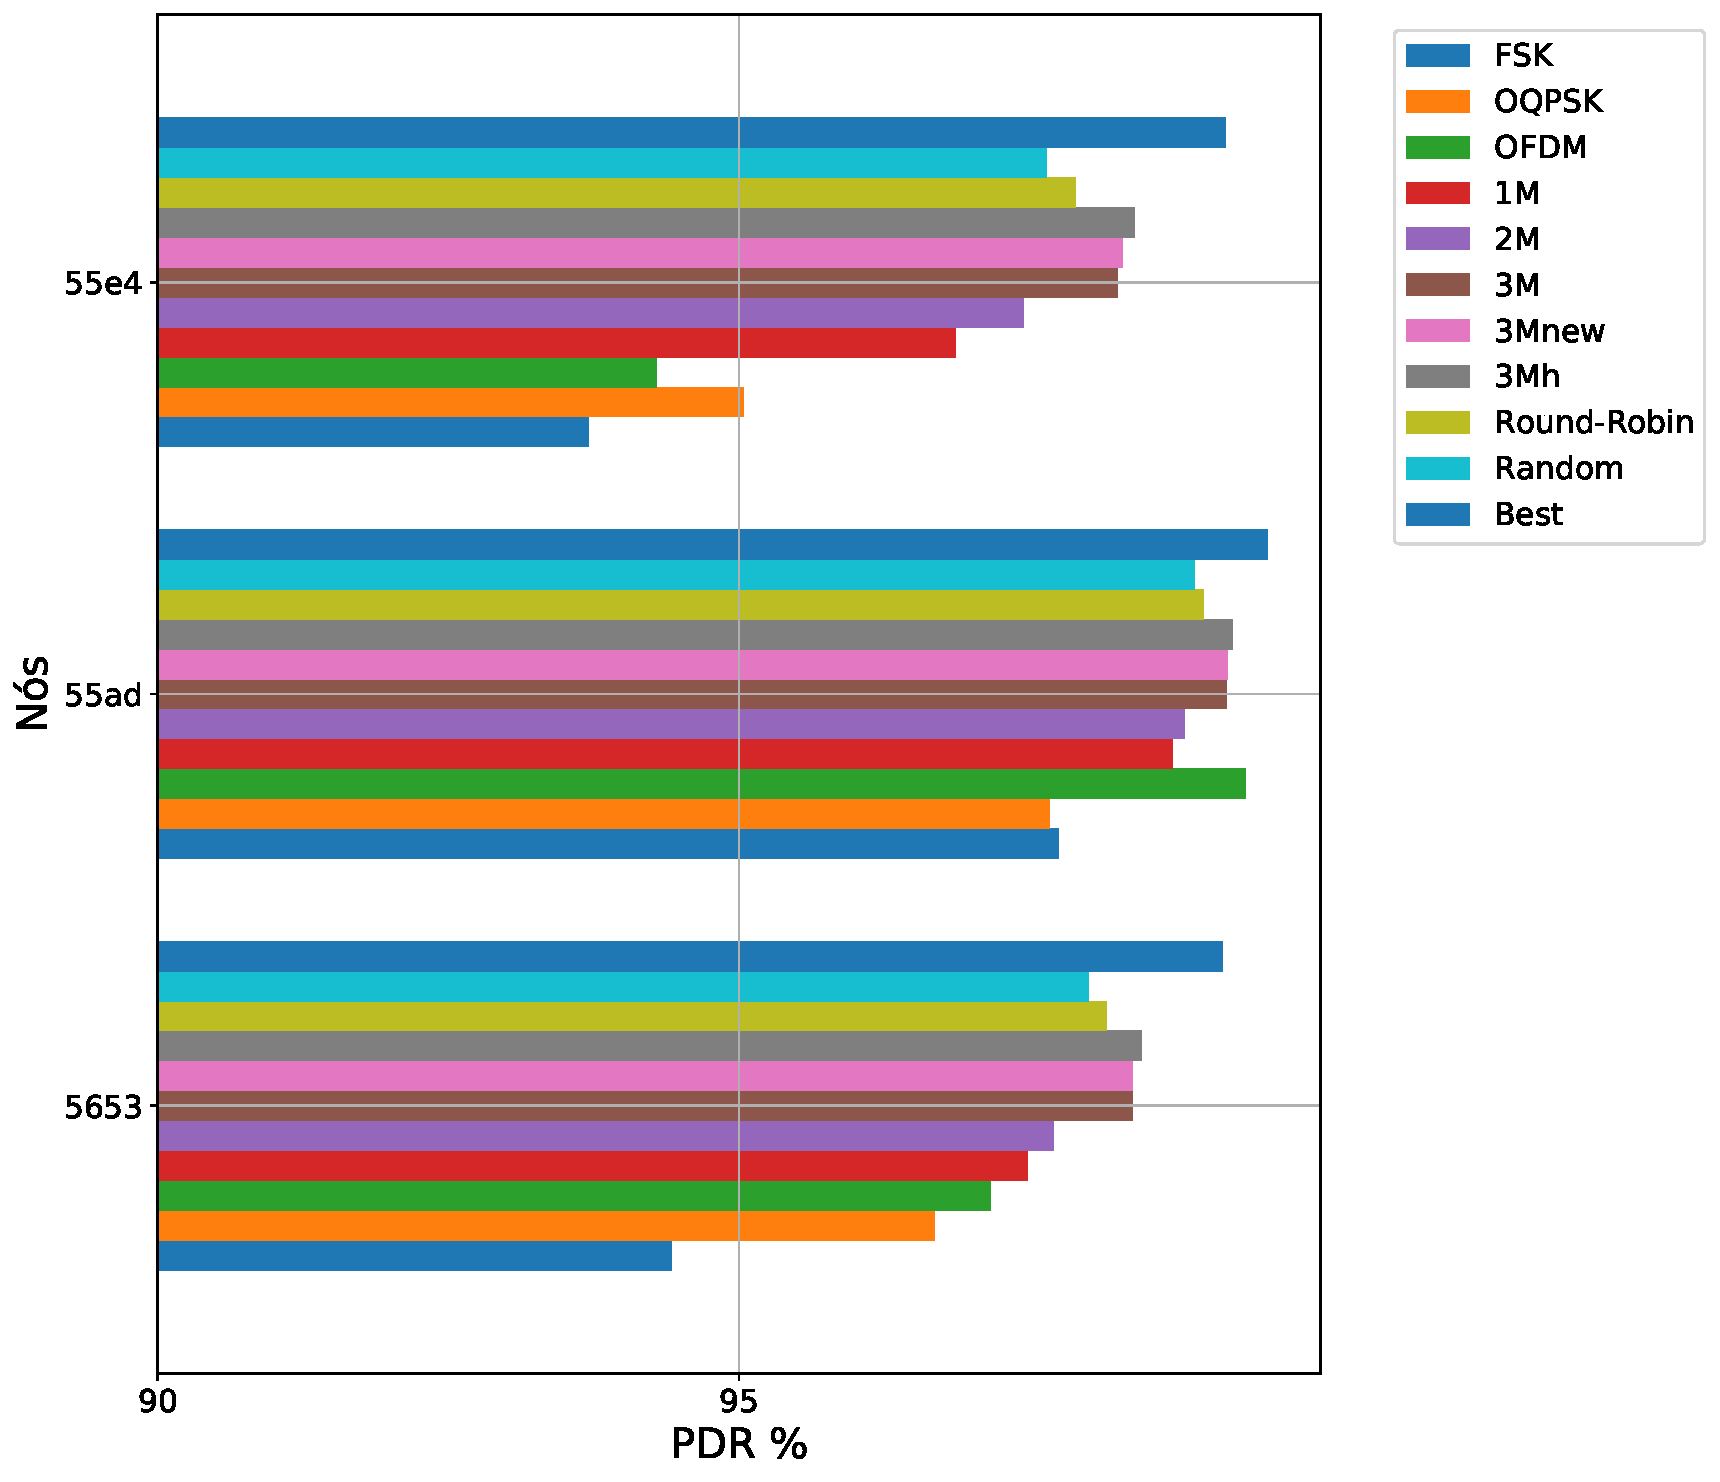
\includegraphics[scale = 0.6]{sections/textual/Imagens/grupo1.pdf}\\
    Fonte: Autoria própia
    \label{fig:g1}
\end{figure}

\begin{figure}[H]
    \centering
    \caption{\footnotesize PDR dos nós que estão no Grupo 2.}
    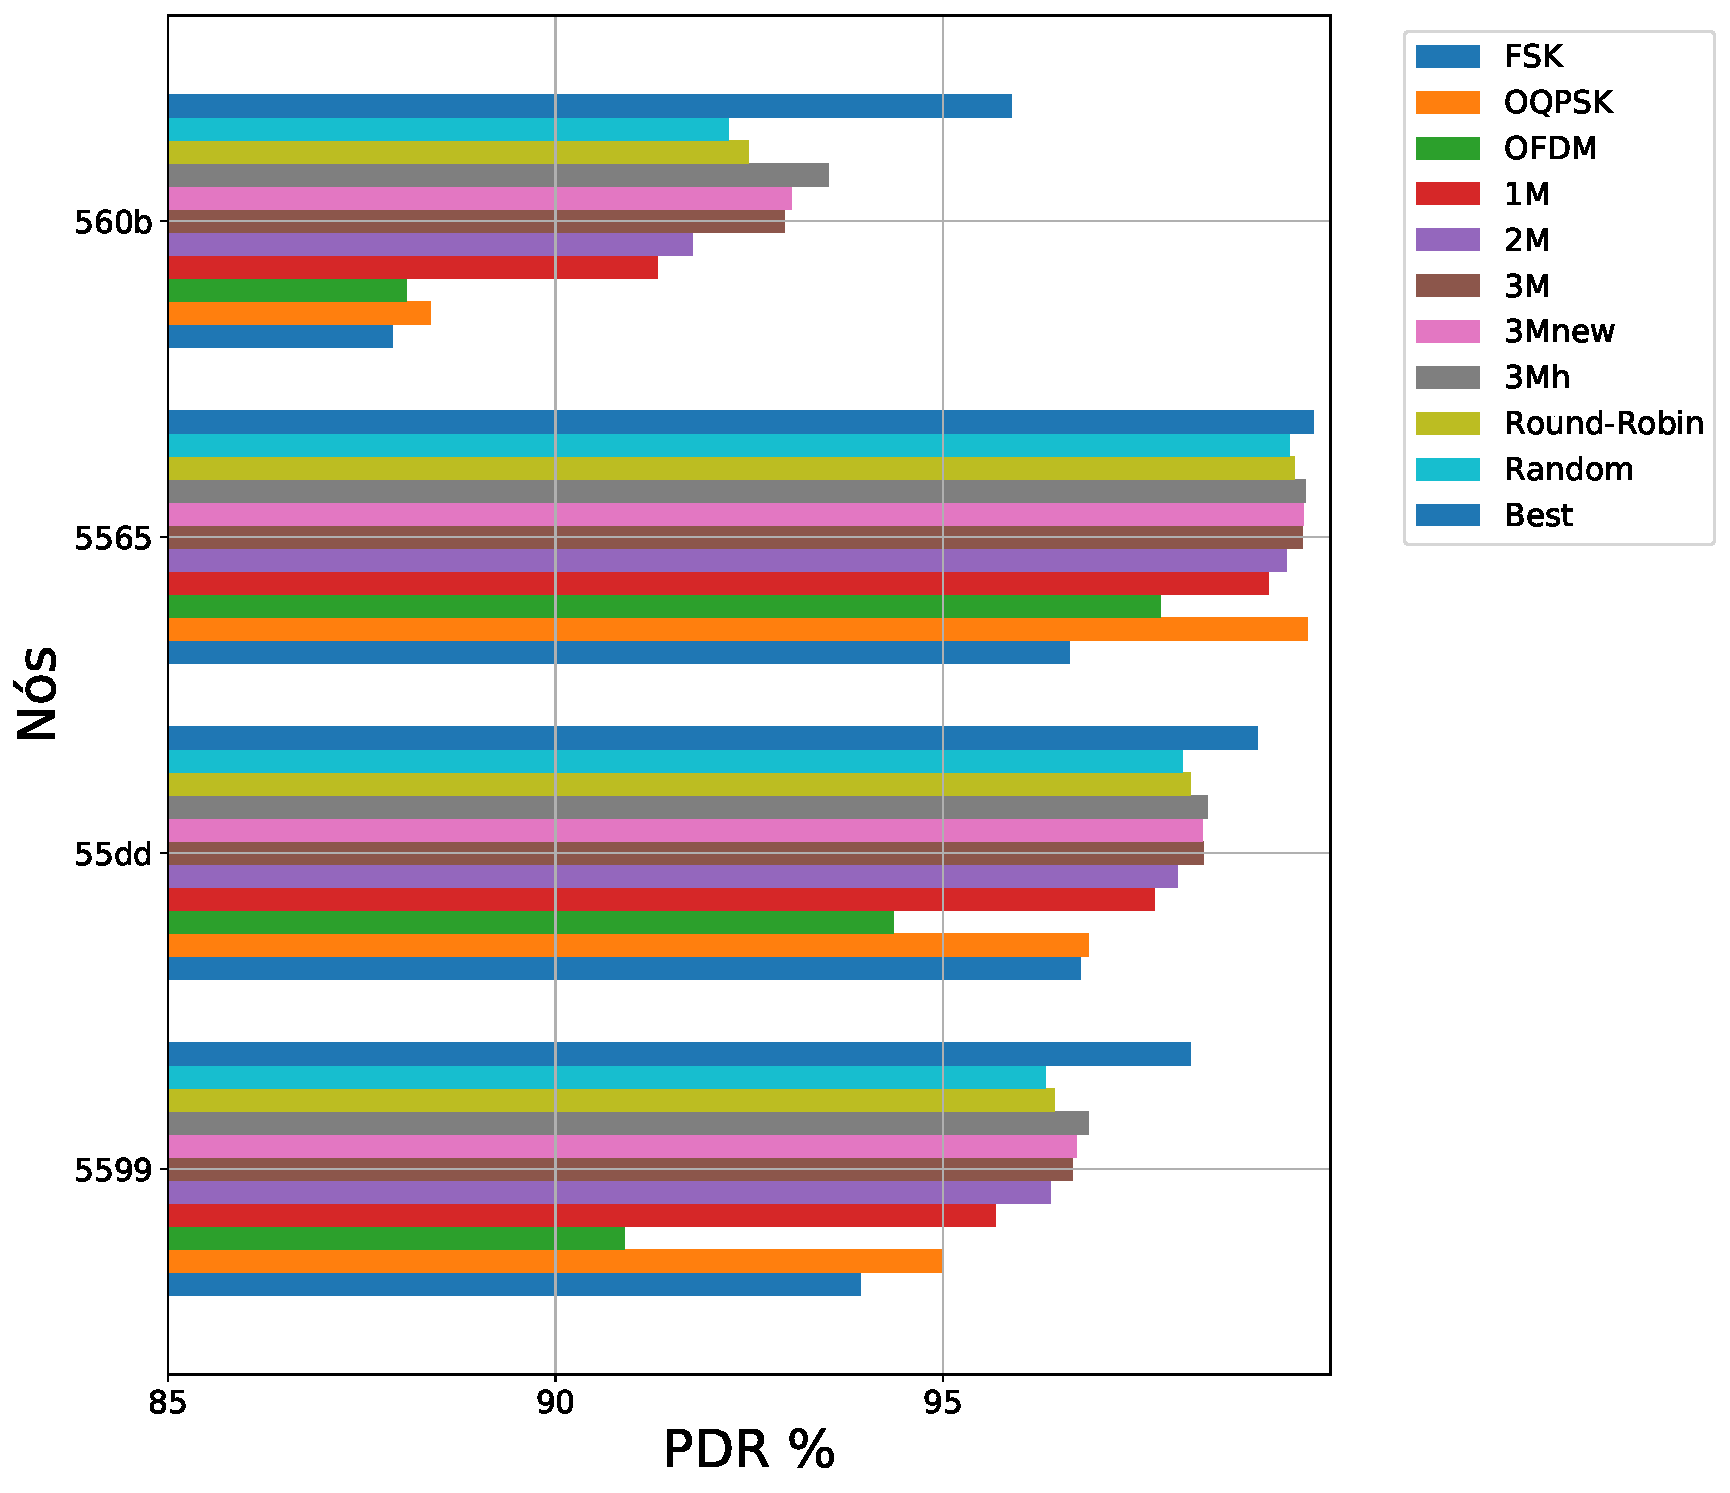
\includegraphics[scale = 0.6]{sections/textual/Imagens/grupo2.pdf}\\
    Fonte: Autoria própia
    \label{fig:g2}
\end{figure}

\begin{figure}[H]
    \centering
    \caption{\footnotesize PDR dos nós que estão no Grupo 3.}
    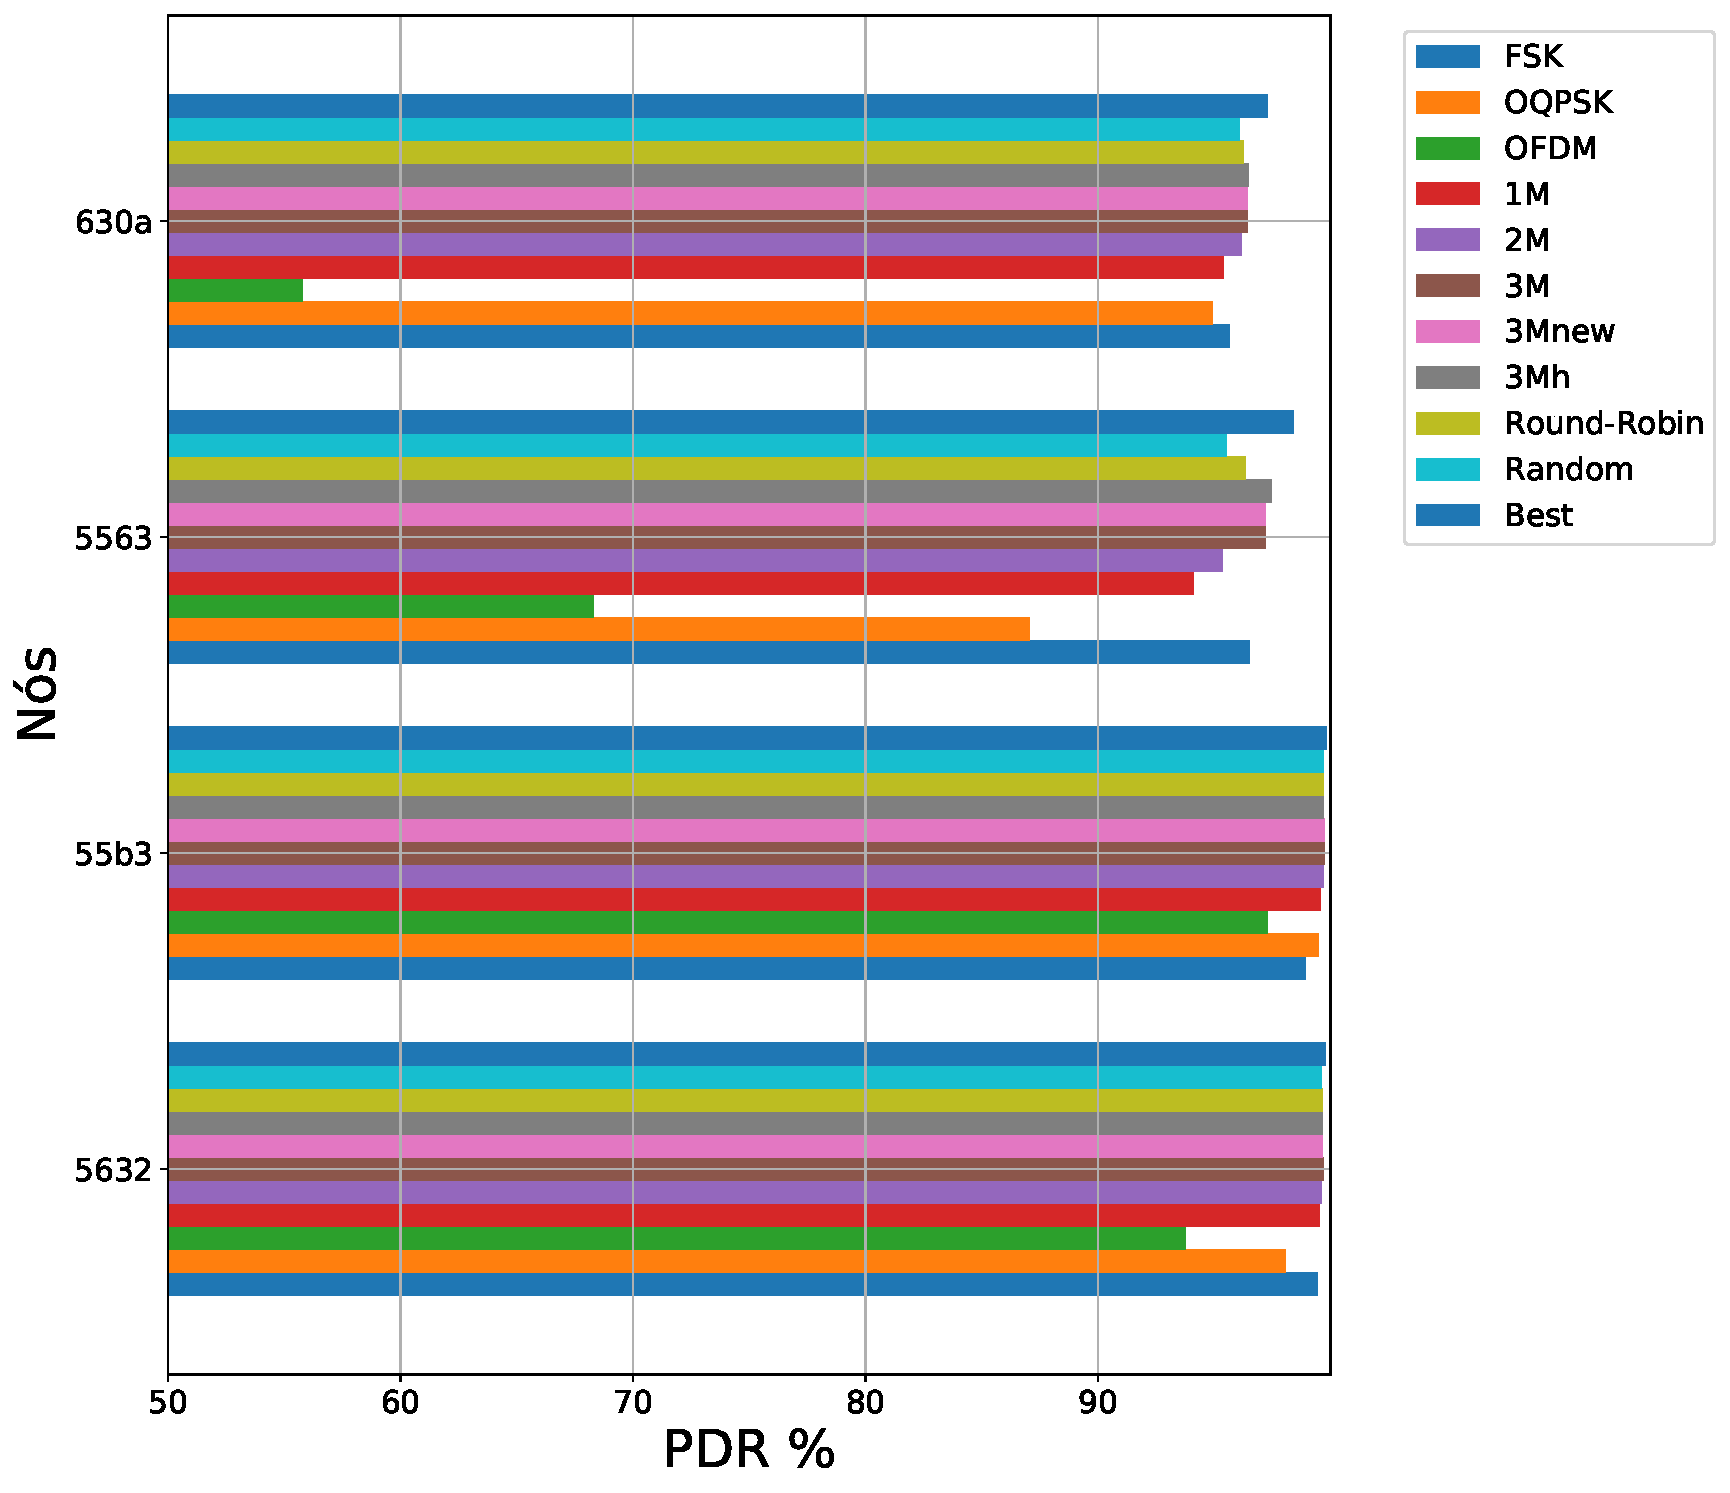
\includegraphics[scale =0.6]{sections/textual/Imagens/grupo3.pdf}\\
    Fonte: Autoria própia
    \label{fig:g3}
\end{figure}

\newpage
Segue a tabela com os valores calculados de cada estratégia, \ref{tabela:pdr} com os valores do PDR médio e \ref{tabela:rnp} com os valores do RNP médio. 

\begin{table}[H]
\centering
\begin{tabular}{l|lll|llll|llll|}
\cline{2-12}
 &
  \multicolumn{1}{l|}{5653} &
  \multicolumn{1}{l|}{55ad} &
  55e4 &
  \multicolumn{1}{l|}{5599} &
  \multicolumn{1}{l|}{55dd} &
  \multicolumn{1}{l|}{5565} &
  560b &
  \multicolumn{1}{l|}{5632} &
  \multicolumn{1}{l|}{55b3} &
  \multicolumn{1}{l|}{5563} &
  630a \\ \hline
\multicolumn{1}{|l|}{FSK}    & 94.42 & 97.74 & 93.71 & 93.93 & 96.77 & 96.63 & 87.89 & 99.44 & 98.92 & 96.52 & 95.67 \\ \cline{1-1}
\multicolumn{1}{|l|}{OQPSK}  & 96.68 & 97.67 & 95.03 & 95.01 & 96.88 & 99.70 & 88.39 & 98.07 & 99.49 & 87.04 & 94.95 \\ \cline{1-1}
\multicolumn{1}{|l|}{OFDM}   & 97.16 & 99.36 & 94.29 & 90.88 & 94.36 & 97.81 & 88.08 & 93.75 & 97.30 & 68.30 & 55.77 \\ \cline{1-1}
\multicolumn{1}{|l|}{1M}     & 97.48 & 98.72 & 96.86 & 95.68 & 97.73 & 99.20 & 91.32 & 99.51 & 99.59 & 94.11 & 95.40 \\ \cline{1-1}
\multicolumn{1}{|l|}{2M}     & 97.71 & 98.83 & 97.44 & 96.39 & 98.02 & 99.44 & 91.77 & 99.62 & 99.69 & 95.35 & 96.16 \\ \cline{1-1}
\multicolumn{1}{|l|}{3M}     & 98.39 & 99.20 & 98.25 & 96.67 & 98.36 & 99.63 & 92.96 & 99.68 & 99.75 & 97.19 & 96.45 \\ \cline{1-1}
\multicolumn{1}{|l|}{3Mnew}  & 98.38 & 99.20 & 98.30 & 96.73 & 98.35 & 99.65 & 93.04 & 99.68 & 99.75 & 97.19 & 96.44 \\ \cline{1-1}
\multicolumn{1}{|l|}{3Mh}    & 98.46 & 99.24 & 98.40 & 96.88 & 98.41 & 99.67 & 93.53 & 99.64 & 99.72 & 97.46 & 96.46 \\ \cline{1-1}
\multicolumn{1}{|l|}{\begin{tabular}[c]{@{}l@{}}Round\\ Robin\end{tabular}} &
  98.16 &
  99.00 &
  97.89 &
  96.44 &
  98.19 &
  99.54 &
  92.49 &
  99.65 &
  99.72 &
  96.36 &
  96.27 \\ \cline{1-1}
\multicolumn{1}{|l|}{Random} & 98.00 & 98.92 & 97.65 & 96.32 & 98.09 & 99.47 & 92.24 & 99.60 & 99.71 & 95.54 & 96.08 \\ \cline{1-1}
\multicolumn{1}{|l|}{Best}   & 99.16 & 99.55 & 99.19 & 98.20 & 99.06 & 99.79 & 95.88 & 99.79 & 99.83 & 98.40 & 97.31 \\ \hline
\end{tabular}
\caption{PDR(\%) Médio }
\label{tabela:pdr}
\end{table}

\begin{table}[H]
\centering
\begin{tabular}{c|ccc|cccc|cccc|}
\cline{2-12}
                             & 5653 & 55ad & 55e4 & 5599 & 55dd & 5565 & 560b & 5632 & 55b3 & 5563 & 630a \\ \hline
\multicolumn{1}{|c|}{FSK}    & 2.39 & 1.89 & 2.57 & 2.02 & 1.50 & 1.81 & 2.31 & 1.18 & 1.41 & 1.61 & 1.69 \\ \cline{1-1}
\multicolumn{1}{|c|}{OQPSK}  & 2.11 & 1.96 & 2.36 & 2.06 & 1.52 & 1.39 & 2.29 & 1.42 & 1.36 & 2.30 & 1.80 \\ \cline{1-1}
\multicolumn{1}{|c|}{OFDM}   & 2.42 & 1.66 & 2.70 & 3.33 & 2.07 & 1.96 & 3.40 & 2.01 & 2.08 & 3.41 & 4.97 \\ \cline{1-1}
\multicolumn{1}{|c|}{1M}     & 1.99 & 1.68 & 2.07 & 2.07 & 1.46 & 1.51 & 2.24 & 1.20 & 1.33 & 1.68 & 1.72 \\ \cline{1-1}
\multicolumn{1}{|c|}{2M}     & 2.05 & 1.73 & 2.17 & 2.24 & 1.51 & 1.57 & 2.27 & 1.27 & 1.34 & 1.81 & 1.81 \\ \cline{1-1}
\multicolumn{1}{|c|}{3M}     & 1.87 & 1.59 & 1.92 & 1.96 & 1.42 & 1.43 & 2.14 & 1.81 & 1.30 & 1.56 & 1.62 \\ \cline{1-1}
\multicolumn{1}{|c|}{3Mnew}  & 1.87 & 1.59 & 1.91 & 1.95 & 1.42 & 1.43 & 2.13 & 1.18 & 1.31 & 1.56 & 1.62 \\ \cline{1-1}
\multicolumn{1}{|c|}{3Mh}    & 1.87 & 1.59 & 1.91 & 1.95 & 1.42 & 1.43 & 2.13 & 1.18 & 1.31 & 1.56 & 1.62 \\ \cline{1-1}
\multicolumn{1}{|c|}{\begin{tabular}[c]{@{}c@{}}Round\\ Robin\end{tabular}} & 2.11 & 1.75 & 2.27 & 2.21 & 1.55 & 1.59 & 2.40 & 1.33 & 1.45 & 2.01 & 2.06 \\ \cline{1-1}
\multicolumn{1}{|c|}{Random} & 2.11 & 1.75 & 2.26 & 2.21 & 1.54 & 1.59 & 2.39 & 1.32 & 1.45 & 1.99 & 2.05 \\ \cline{1-1}
\multicolumn{1}{|c|}{Best}   & 1.63 & 1.43 & 1.68 & 1.79 & 1.33 & 1.31 & 2.00 & 1.13 & 1.12 & 1.42 & 1.54 \\ \hline

\end{tabular}
\caption{RNP(\%) médio}
\label{tabela:rnp}
\end{table}


A Figura \ref{fig:pdrglobal} mostra o pdr global das estratégias. Pode-se observar que a atualização proposta na estratégia 3M, a 3Mh, consegue um PDR global superior.

\begin{figure}[H]
    \centering
    \caption{\footnotesize PDR global}
    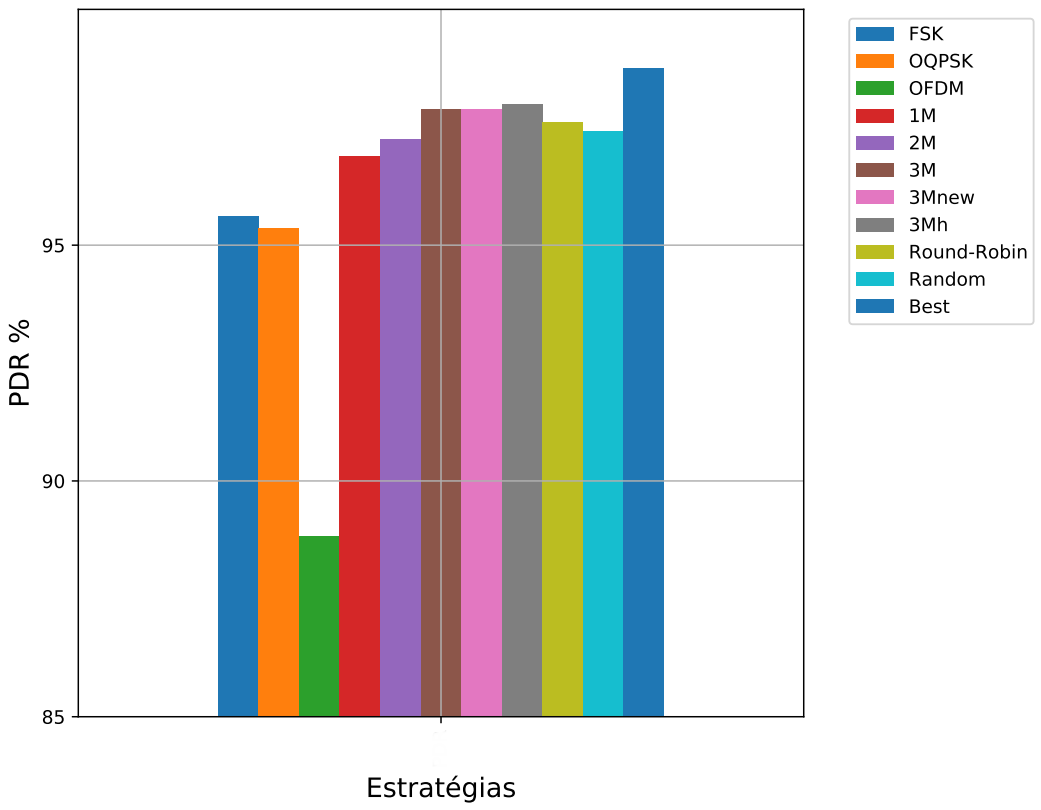
\includegraphics[scale = 0.6]{sections/textual/Imagens/pdrglobal.png}\\
    Fonte: Autoria própia
    \label{fig:pdrglobal}
\end{figure}


\newpage

Como mencionando anteriormente, foi permitido o uso de até 6 retransmissões de cada pacote, caso o mesmo seja perdido. Essa técnica de replicação de pacotes consegue de certo modo aumentar o PDR, mas dependendo de como for usada, pode ter um impacto significativo. Se é necessário realizar várias retransmissões para que um pacote seja enviado, isso significa que o canal de comunicação não está sendo usado de forma eficiente e consequentemente, aumenta o consumo de energia nos nós, além de sobrecarregar a rede. Essa sobrecarga pode vir a atrapalhar tanto a durabilidade, tendo em vista que esses nós em grande parte são alimentados por baterias, tanto quanto sua escalabilidade, dificultando futuras expansões na rede caso essa sobrecarga seja mantida. 

A Figura \ref{fig:pdrvsrnp} mostra um comparativo da RNP e o PDR para as diferentes estratégias de diversidade de modulação adaptativa. Cada cor da linha representa uma estratégia de diversidade de modulação e cada ponto representa o número de retransmissões permitidas para essa estratégia, nesse caso, de 1 a 9. É possível notar que permitir mais retransmissões aumenta de forma significativa o PDR alcançado, mas em um determinado ponto, o aumento do PDR vai ficando cada vez menor. Também é possível observar que a estratégia 3Mh consegue reduzir ligeiramente a quantidade de transmissões requeridas para um mesmo nível de PDR. Apesar da \textit{Round-Robin} conseguir um PDR global próximo das estratégias 3M, 3M\textit{new} e 3Mh, é possível notar que o valor da RNP é bem superior. 

\begin{figure}[H]
    \centering
    \caption{\footnotesize RNP e PDR - Cada ponto representa o número de retransmissões de pacotes permitidas para essa estrategia específica, de 1 a 9}
    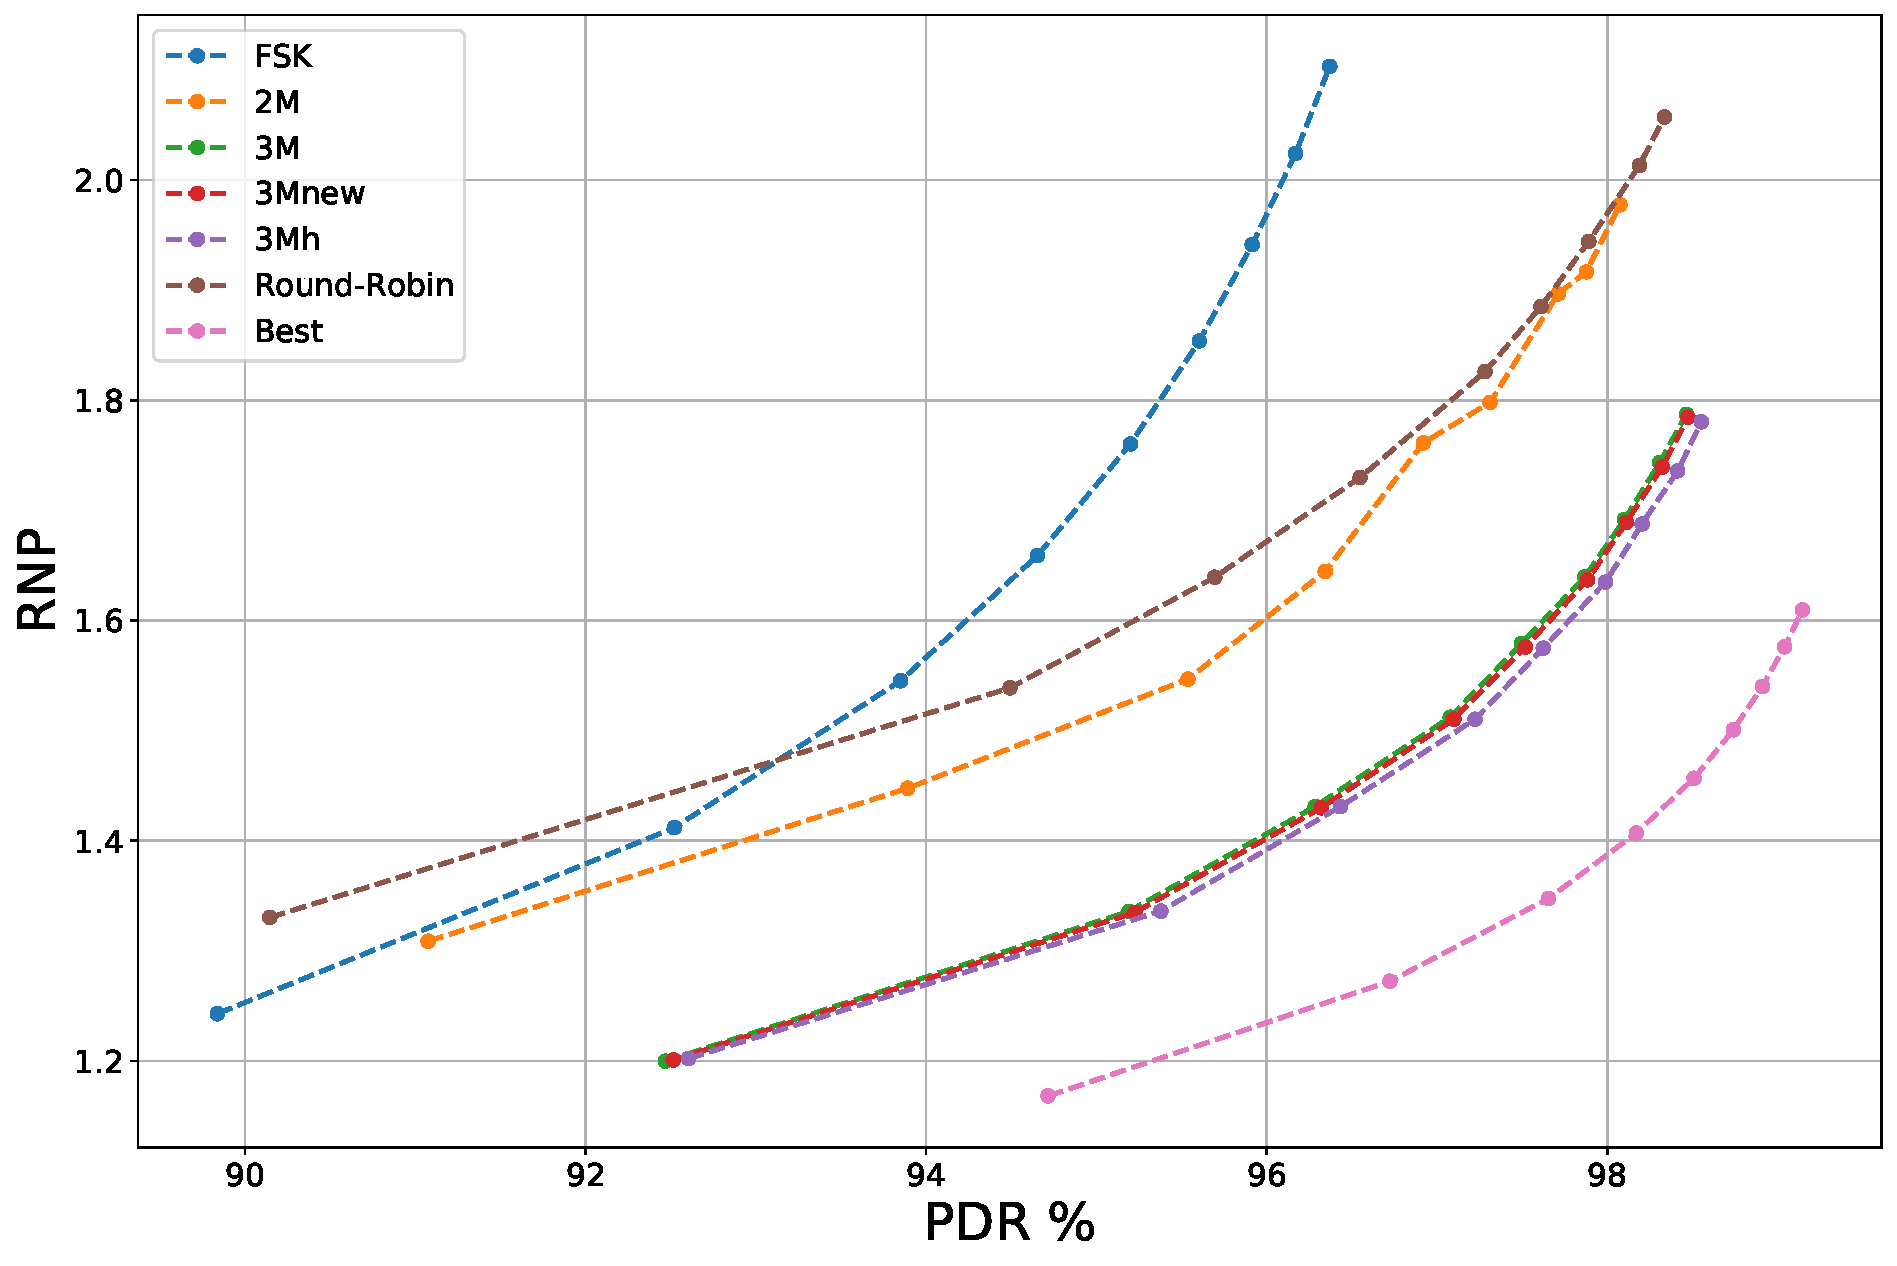
\includegraphics[scale = 0.5]{sections/textual/Imagens/pdrvsrnp.pdf}\\
    Fonte: Autoria própia
    \label{fig:pdrvsrnp}
\end{figure}



 % Capítulos

% ---
% Finaliza a parte no bookmark do PDF
% para que se inicie o bookmark na raiz
% e adiciona espaço de parte no Sumário
% ---

%\phantompart

% Conclusão (outro exemplo de capítulo sem numeração e presente no sumário)
\chapter{Considerações Finais}
\label{cap:conlusao}

Este trabalho propôs duas novas estratégias de estimação de qualidade de enlace, que foram aplicadas em um mecanismo de seleção de modulação em redes IEEE 802.15.4g. Os resultados obtidos mostram que a primeira estratégia proposta, 3M\textit{new}, consegue fornecer uma estimativa de qualidade de enlace superior em relação ao estimador do estado da arte (3M). A maior contribuição dessa estratégia foi a possibilidade de obter uma melhor estimação da qualidade do enlace, usando as informações calculadas no receptor. 

A partir desta estimação mais precisa, foi possível a criação de uma estratégia híbrida, a 3Mh, que utiliza de forma híbrida os valores do ARR combinados com o PRR utilizando pesos iguais. A estratégia 3Mh conseguiu um PDR superior em 9 dos 11 nós e um PDR global superior em relação as estratégias 3M e 3M\textit{new}. 

\section{Sugestões para Trabalhos Futuros}

Como sugestões de trabalhos futuros:
\begin{itemize}
    \item Avaliar outros mecanismos de estimação de qualidade do enlace;
    \item O uso de outros protocolos para a escolha dinâmica de modulação;
    \item Realização de testes em outros cenários, bem como a realização de novos experimentos em ambientes industriais reais;
    \item Fazer os comparativos do PDR médio e RNP médio, talvez seja possível criar um preditor, achando uma correlação entre as duas variáveis. Caso essa correlação seja encontrada, é possível usar uma variável para prever a outra;
    \item A partir dos valores de similaridade, alterar os pesos utilizados no 3Mh. Utilizando uma estratégia inteligente que consiga usar o melhor estimador em determinando momento, alterando o peso do estimador com melhor precisão.  
\end{itemize}




% ---
% ELEMENTOS PÓS-TEXTUAIS
% ---
\postextual

\bibliography{./referencia}        % Referências bibliográficas

% ---
% Glossário
% Consulte o manual da classe abntex2 para orientações sobre o glossário.
% \glossary

%\begin{apendicesenv}
  \partapendices  % Imprime uma página indicando o início dos apêndices

  \chapter{Um Apêndice}
  \label{ape:apendiceI}
  Para criar um novo apêndice utilize o comando chapter, lembre de utilizar label para referenciar.

\end{apendicesenv}
   % Apêndices
%\begin{anexosenv}
  \partanexos % Imprime uma página indicando o início dos anexos

  \chapter{Um Anexo}
  \label{ape:anexoI}
  Para criar um novo anexo utilize o comando chapter, lembre de utilizar label para referenciar.


\end{anexosenv}
      % Anexos

%---
% INDICE REMISSIVO
% \phantompart
\printindex

\end{document}
